\section{Sistemi Composti}

	Si consideri un sistema di due particelle $1$ e $2$. Sia $\mathcal{H}_1$ lo spazio degli stati della particella $1$ e $\mathcal{H}_2$ lo spazio degli stati della particella $2$. Sia invece $\mathcal{H}$ lo spazio degli stati del sistema composto. 
	\\
	\\
	Mi chiedo allora quale sia la relazione tra gli spazi:
	\\
	\\
	Siano allora:
	
\begin{align*}
	\qty{ \ket{\lambda_i}, \, \, i =1, \ldots, m } \qquad \text{e} \qquad \qty{ \ket{\mu_{\alpha}}, \, \, \alpha =1, \ldots, n }
\end{align*}

	rispettivamente basi di $\mathcal{H}_1$ e $\mathcal{H}_2$. Definisco:
	
\begin{mydef}
	Sia il \textbf{prodotto tensoriale} tra i due spazi $\mathcal{H}_1$ e $\mathcal{H}_2$ il seguente prodotto:
	
\begin{align*}
	\mathcal{H} = \mathcal{H}_1 \otimes \mathcal{H}_2
\end{align*}

	con base:
	
\begin{align*}
	\qty{ \ket{\lambda_i} \otimes \ket{\mu_{\alpha}}  \, \equiv \, \ket{\lambda_i, \mu_{\alpha}} \, \equiv \, \ket{\lambda_i} \ket{\mu_{\alpha}} }
\end{align*}

	di $m \times n$ elementi.

\end{mydef}

	Pertanto vale che:

\begin{nb}
\begin{align*}
	\forall v \in \mathcal{H}_1 \otimes \mathcal{H}_2 \quad \text{allora} \quad v = \sum_{i, \alpha} c_{i\alpha} \ket{\lambda_i} \ket{\mu_{\alpha}}
\end{align*}
\end{nb}

	Vettori di questo tipo permettono di parlare del sistema composto e non dei singoli sottosistemi e vengono chiamati \textbf{entangled states}. La definizione di $v$ è tuttavia ambigua poiché dipende dalla base scelta. Scegliendo però altre basi per $\mathcal{H}_1$ e $\mathcal{H}_2$ otterrei lo stesso spazio tensore $\mathcal{H}$ ma cambierrebbe la rappresentazione degli elementi che lo compongono, cioè la forma esplicita dei vettori nella nuova base. In particolare se prendessimo:
	
\begin{empheq}[left = \empheqlbrace]{align*}
	& \ket{\lambda_i} = M_{ij} \ket{\tilde{\lambda}_j} \\
	& \ket{\mu_{\alpha}} = N_{\alpha \beta} \ket{\tilde{\mu}_{\beta}}
\end{empheq}

	allora avremmo:
	
\begin{align*}
	v = \sum c_{i \alpha} \ket{\lambda_i} \ket{\mu_{\alpha}} = \sum c_{i \alpha} \, M_{ij} N_{\alpha \beta} \ket{\tilde{\lambda}_j}  \ket{\tilde{\mu}_{\beta}} = \sum \tilde{c}_{j \beta} \ket{\tilde{\lambda}_j}  \ket{\tilde{\mu}_{\beta}}
\end{align*}

	abbiamo esplicitato allora che:
	
\begin{itemize}
	\item lo spazio non cambia (è sempre $ \mathcal{H}_1 \otimes \mathcal{H}_2$),
	\item ma le coordinate (cioè i coefficienti $c_{i\alpha}$) cambiano quando si cambia base.
\end{itemize}

\begin{myapprf}
	\textbf{Interpretazione della trasformazione dei coefficienti $c_{i \alpha} \to  \tilde{c}_{j \beta}$}:
	\\
	\\
	Quando si cambia base nei sottospazi $\mathcal{H}_1$ e $ \mathcal{H}_2$, le componenti del vettore $v$ nel prodotto tensoriale cambiano in modo coerente con la trasformazione lineare applicata a ciascun sottospazio. Quindi nel nostro caso:
\begin{empheq}[left = \empheqlbrace]{align*}
	& \ket{\lambda_i} = M_{ij} \ket{\tilde{\lambda}_j} \\
	& \ket{\mu_{\alpha}} = N_{\alpha \beta} \ket{\tilde{\mu}_{\beta}}
\end{empheq}
	i coefficienti si trasformano come:
\begin{align*}
	\tilde{c}_{j \beta} = \sum_{i, \alpha} M_{ij} N_{\alpha \beta} c_{i \alpha}
\end{align*}
	Questa è una trasformazione bilineare: ogni coefficiente si trasforma con una matrice per ogni indice, come nei tensori di rango $2$. Significa che la matrice dei coefficienti $c$ si trasforma secondo:
\begin{align*}
	\tilde{C} = M^TCN
\end{align*}
	dove:
\begin{itemize}
	\item $C$ è la matrice dei coefficienti originali,
	\item $M, N$  sono i cambi di base nei due sottospazi,
	\item $\tilde{C}$ è la nuova matrice dei coefficienti nella base trasformata.
\end{itemize}

	Questa trasformazione evidenzia che:
	
\begin{itemize}
	\item Lo stato fisico del sistema $v$ non cambia (rimane lo stesso vettore nello spazio tensore).
	\item La rappresentazione dello stato cambia con la base: i coefficienti $c_{i \alpha}$ dipendono dalla base scelta, e non sono invarianti.
	\item Tuttavia, le proprietà fisiche del sistema, come il fatto che $v$ sia entangled o separabile, non dipendono dalla base. Infatti, l’entanglement è una proprietà geometrica dello stato, non della sua rappresentazione.
\end{itemize}


\end{myapprf}


	Inoltre vale che:
	
\begin{nb}

	Se le \textit{basi} scelte per i due spazi sono \textit{ortonormali} allora:
	
\begin{align*}
	\braket{\lambda_i \mu_{\alpha}}{\lambda_j \mu_{\beta}} = \braket{\lambda_i}{\lambda_j} \braket{\mu_{\alpha}}{\mu_{\beta}}
\end{align*}

\end{nb}

	È importante osservare che i prodotti di autovettori sono sempre vettori di $\mathcal{H}_1 \otimes \mathcal{H}_2$, ma non tutti i vettori di $\mathcal{H}_1 \otimes \mathcal{H}_2$ sono prodotti di autovettori, ma piuttosto combinazioni di prodotti di vettori dei due spazi.
	\\
	\\
	Che relazione ho tra gli operatori che agiscono su $\mathcal{H}_1$, su $\mathcal{H}_2$ e su $\mathcal{H}_1 \otimes \mathcal{H}_2$?

\begin{nb}
	Definiamo allora i seguenti operatori:

\begin{align*}
	& \hat{O}_1 : \mathcal{H}_1 \to \mathcal{H}_1 \quad \text{tale che} \quad \hat{O}_1 \ket{\lambda_i} = \qty\big(\hat{O}_1)_{ij} \ket{\lambda_j} \\
	& \hat{O}_2 : \mathcal{H}_2 \to \mathcal{H}_2 \quad \text{tale che} \quad \hat{O}_2 \ket{\mu_{\alpha}} = \qty\big(\hat{O}_2)_{\alpha \beta} \ket{\mu_{\beta}} \\
	& \hat{O}_1 \otimes \hat{O}_2 : \mathcal{H} \to \mathcal{H}
\end{align*}
\end{nb}

	allora vale che:
	
\begin{align*}
	\qty\big(\hat{O}_1 \otimes \hat{O}_2) \ket{\lambda_i} \ket{\mu_{\alpha}} = \qty\big(\hat{O}_1 \ket{\lambda_i}) \otimes \qty\big(\hat{O}_2 \ket{\mu_{\alpha}}) =  \qty\big(\hat{O}_1)_{ij} \qty\big(\hat{O}_2)_{\alpha \beta} \ket{\lambda_j} \otimes \ket{\mu_{\beta}}
\end{align*}

	ricordiamo che per definizione vale:
	
\begin{align*}
	\ket{\lambda_j} \otimes \ket{\mu_{\beta}} \, \equiv \, \ket{\lambda_j}\ket{\mu_{\beta}} 
\end{align*}

	allora:
	
\begin{align*}
	\qty\big(\hat{O}_1 \otimes \hat{O}_2) \ket{\lambda_i} \ket{\mu_{\alpha}} = \qty\big(\hat{O}_1)_{ij} \qty\big(\hat{O}_2)_{\alpha \beta} \ket{\lambda_j}\ket{\mu_{\beta}}
\end{align*}

	vale anche che:
	
\begin{align*}
	\qty\big(\hat{O}_1)_{ij} \qty\big(\hat{O}_2)_{\alpha \beta} = \qty(\hat{O}_1 \otimes \hat{O}_2)_{\qty(j\alpha) \qty(i \beta)}
\end{align*}

	Possiamo scrivere infine:
	
\begin{align*}
	\qty\big(\hat{O}_1 \otimes \hat{O}_2) \ket{\lambda_i} \ket{\mu_{\alpha}} = \qty(\hat{O}_1 \otimes \hat{O}_2)_{\qty(j\alpha) \qty(i \beta)} \ket{\lambda_j} \ket{\mu_{\beta}}
\end{align*}

\subsection{Osservazioni:}

\begin{enumerate}[label=\arabic*)]

	\item $\forall \hat{O}: \hat{O}_1 \otimes \hat{O}_2 \to \hat{O}_1 \otimes \hat{O}_2$ vale che l'algebra è tale che  qualunque operatore si può scrivere come combinazione lineare dei prodotti tensori relativi (\textbf{entanglement})
	\begin{align*}
		\hat{O} = \sum \qty(\hat{A} \otimes \hat{B})
	\end{align*}
		stiamo dicendo che ogni operatore $\hat{O}_1 \otimes \hat{O}_2 $ può essere scritto come combinazione lineare di operatori del tipo $\hat{A} \otimes \hat{B}$, dove:
	\begin{itemize}
		\item $\hat{A}$ agisce su $\mathcal{H}_1$.
		\item $\hat{B}$ agisce su $\mathcal{H}_2$.
	\end{itemize}
 	
		ma chi sono nello specifico? Vediamolo nella prossima osservazione.
	
	\item Esistono degli operatori "naturali" che agiscono sui singoli fattori. Siano infatti:
	\begin{align*}
		\hat{A} : \mathcal{H}_1 \to \mathcal{H}_2 \qquad ; \qquad \hat{B} : \mathcal{H}_2 \to \mathcal{H}_2
	\end{align*}
	
		e definisco allora come:
		
	\begin{align*}
		& \hat{\mathcal{A}} \, \equiv \, \hat{A} \otimes \mathbb{I} \, \, \Rightarrow \,\, \hat{\mathcal{A}} v \otimes w = \qty\big(\hat{A} v) \otimes w \\
		& \hat{\mathcal{B}} \, \equiv \,  \mathbb{I} \otimes \hat{B} \, \, \Rightarrow \,\, \hat{\mathcal{B}} v \otimes w = v \otimes \qty\big(\hat{B} w) 
	\end{align*}
	
		che rispettivamente agiscono solo sul primo e sul secondo fattore. Per queste loro proprietà $\hat{\mathcal{A}}$ e $\hat{\mathcal{B}}$ vengono chiamati \textbf{operatori di singola particella}. Essi commutano infatti:
	\begin{empheq}[left = \empheqlbrace]{align*}
		& \hat{\mathcal{A}} \hat{\mathcal{B}} = \qty(\hat{A} \otimes \mathbb{I}) \, \qty(\mathbb{I} \otimes \hat{B}) = \hat{A} \otimes \hat{B} \\
		& \hat{\mathcal{B}} \hat{\mathcal{A}} =  \qty(\mathbb{I} \otimes \hat{B}) \, \qty(\hat{A} \otimes \mathbb{I})= \hat{A} \otimes \hat{B}
	\end{empheq}
	
		ne segue allora che:
		
	\begin{align*}
		\Rightarrow \, \qty[\hat{\mathcal{A}}, \hat{\mathcal{B}}] = 0
	\end{align*}
	
		in questo modo, la versione formalmente corretta dell'espressione del momento angolare è:
	
	\begin{mydef}
	\begin{align*}
		\hat{J}_i = \hat{L}_i \otimes \mathbb{I} + \mathbb{I} \otimes \hat{S}_i
	\end{align*}
	\end{mydef}

	
\end{enumerate}
	
	Che applicazioni ho di tutto ciò?
	\\
	\\
	Sia $\mathcal{H}_1 = L_2\qty(\mathbb{R}^3)$, lo spazio di una particella che si muove in $\mathbb{R}^3$. Una base di autostati impropri può essere $\qty{\ket{\vb{x}}}$ ad esempio. In questa base qualunque stato è rappresentato come funzione delle coordinate:
	
\begin{align*}
	\Psi\qty(\vb{x}) = \braket{\vb{x}}{\Psi}
\end{align*}

	dunque ho $3$ osservabili $\vb{\hat{x}} = \qty(\hat{x}_1, \hat{x}_2, \hat{x}_3) $ che formano un insieme completo, ossia un \textbf{sistema puntiforme}: fissate le tre osservabili ho una degenerazione finita, cioè una \textbf{particella puntiforme}. Ciò significa che lo spazio che la descrive non è $\mathcal{H}_1$, bensì:
	
\begin{align*}
	\mathcal{H} = L_2 \qty(\mathbb{R}^3) \otimes \mathcal{H}_J \qquad \text{con : }  \, \,\,\, \dim \mathcal{H}_J = 2 J + 1
\end{align*}

	per questo motivo, una base del sistema è data da: $\ket{\vb{\hat{x}}} \otimes \ket{\sigma}$, con $\sigma = \qty{-s, \ldots, + s}$, quindi uno stato è dato da una \textit{coppia di funzioni} del tipo:
	
\begin{align*}
	\braket{\vb{x}, \sigma }{\Psi} = \Psi\qty(\vb{x}, \sigma)
\end{align*}

 	Nel caso dell'elettrone, ad esempio, ho $s = 1/2$, perciò:
	
\begin{align*}
	\Psi(\vb{x}, \sigma) = \mqty( \psi\qty(\vb{x}, 1/2) \\  \psi\qty(\vb{x}, -1/2) ) \, \equiv \, \mqty( \psi_+\qty(\vb{x}) \\\psi_-\qty(\vb{x}) )
\end{align*}

	ed ho che:
	
\begin{align*}
	| \psi_{\pm} (\vb{x}) |^2 \, \dd^3 \vb{x}
\end{align*}

	è la probabilità di trovare l'elettrone con spin $\pm s$ nella regione scelta. Per conoscere la probabilità di trovare l'elettrone in una data regione senza conoscere lo spin, sommo la probabilità nel caso $+s$ con quella del caso $-s$.

\section{Composizione di Momenti Angolari}

	Si supponga di avere due particelle di spin $1/2$, ad esempio un \textit{elettrone} ed un \textit{protone}, nel loro stato fondamentale in modo da, all'inizio, non considerare il momento angolare orbitale. Ogni particella può avere spin \textit{up} oppure spin \textit{down}, quindi ho quattro possibili combinazioni nella rappresentazione degli stati di spin combinato del sistema composto dalle due particelle:
	
\begin{align*}
	\ket{+, +}, \ket{+, -}, \ket{-, +}, \ket{-, -}
\end{align*}

	dove all'interno del \textit{ket} si  il primo termine si riferisce all'elettrone mentre il secondo al protone.
	\\
	\\
	Qual è il momento angolare totale? Mi sto chiedendo quale sia lo spin totale, sia dunque:

\begin{align*}
	\vb*{\hat{S}} = \vb*{\hat{S}}^{\qty(1)} \otimes \mathbb{I} + \mathbb{I} \otimes \vb*{\hat{S}}^{\qty(2)} = \vb*{\hat{S}}^{\qty(1)} + \vb*{\hat{S}}^{\qty(2)}
\end{align*}

	ognuno dei quattro stati composti è un autostato di $\hat{S}_z$, perciò l'azione su degli stati generici è:
	
\begin{align*}
	\hat{S}_z \ket{1} \ket{2} = \qty(\hat{S}_z^{\qty(1)} + \hat{S}_z^{\qty(2)}  ) \ket{1} \ket{2} = \qty(\hat{S}_z^{\qty(1)} \ket{1}) \ket{2} + \ket{1} \qty(\hat{S}_z^{\qty(2)} \ket{2}) = \hbar \qty(m_1 + m_2) \ket{1} \ket{2}
\end{align*}

	quindi ho che $m = m_1 + m_2$:

\begin{align*}
	& \ket{+, +} : m = 1 \\
	& \ket{+, -} : m = 0 \\
	& \ket{-, +} : m = 0 \\
	& \ket{-, -} : m = -1
\end{align*}

	A prima vista può sembrare sbagliato: $m$ ha valori di passo intero da $-s$ a $+s$, con $s = 1$ in questo caso, ma nel calcolo di prima compare uno stato extra con $m = 0$. La soluzione al problema sta nell'applicare l'operatore di discesa $\hat{J}_- = \hat{S}_- = \hat{S}_-^{\qty(1)} + \hat{S}_-^{\qty(2)}$ allo stato $\ket{+, +}$. Infatti:
	
\begin{align*}
	\hat{S}_- \ket{+, +} = \qty(\hat{S}_{-}^{\qty(1)} \ket{+}) \ket{+} + \ket{+} \qty(\hat{S}_{-}^{\qty(2)} \ket{+}) = \qty(\hbar \ket{-}) \ket{+} + \ket{+ }\qty(\hbar \ket{-}) = \hbar \qty(\ket{-, +} + \ket{+, -})
\end{align*}

	ricordando l'azione di $\hat{S}_-$ su $m$ si capisce che, nella notazione $\ket{s, m}$, ho tre stati con $S = 1$:
	
\begin{empheq}[left = \empheqlbrace]{align*}
	& \ket{1, 1} = \ket{+, +} \\
	& \ket{1, 0} = \frac{1}{\sqrt{2}} \,  \qty(\ket{+, -} + \ket{-, +}) \, \, \Rightarrow \, \, S = 1 \, \, \text{(stato di \textit{tripletto})} \\
	& \ket{1, -1} = \ket{-, -}
\end{empheq}

	ed uno stato con $S = 0$:
	
\begin{align*}
	\ket{0, 0} = \frac{1}{\sqrt{2}}\, \qty(\ket{+, -} - \ket{-, +}) \, \, \Rightarrow \, \, S = 0 \, \, \text{(stato di \textit{singoletto})}
\end{align*}

	ricavato semplicemente dato che è l'unico stato ortogonale allo stato tripletto $\ket{1, 0}$.
	\\
	\\
	Un modo più formale per trovare gli stati della composizione di due spin $1/2$ è il seguente: formalmente, la composizione di due spin $1/2$ da:
	
\begin{align*}
	\mathcal{H} = \mathcal{H}_{1/2} \otimes \mathcal{H}_{1/2} = \frac{1}{2} \otimes \frac{1}{2} = 0 \oplus 1
\end{align*}
 
	e poiché vale:
	
\begin{align*}
	\dim \mathcal{H}_0 = 1 \qquad ; \qquad \dim \mathcal{H}_1 = 3
\end{align*}

	mi aspetto di trovare una configurazione di singoletto, con spin totale $S = 0$, ed una con di tripletto, con spin totale $S = 1$. Cerco adesso lo spettro di $\hat{S}_z$: visto che commuta con $\hat{S}_1^2, \hat{S}_2^2, \hat{S}_{1z} $ e $\hat{S}_{2z}$ una sua base è: $\ket{m_1, m_2}$ perciò:
	
\begin{align*}
	& \hat{S}_z \ket{+, +} = \hbar \ket{+, +} \quad ; \quad \hat{S}_z \ket{+, -} = 0 \\
	& \hat{S}_z \ket{-, -} =  - \hbar \ket{-, -} \quad ; \quad \hat{S}_z \ket{-, -} = 0
\end{align*}

	da cui ho gli autovalori: $ m = m_1 + m_2 = -1, 0, 1$. Gli autovalori $\pm 1$ sono non degeneri, mentre l'autovalore $0$ è degenere con degenerazione $2$. Quindi la rappresentazione di $\hat{S}_z$ nella base scelta è:
	
\begin{align*}
	\hat{S}_z = \hbar \mqty( 1 & 0 & 0 & 0 \\ 0 & 0 & 0 & 0 \\ 0 & 0 & 0 & 0 \\ 0 & 0 & 0 & -1)
\end{align*}

	con ordinamento $\qty{\ket{+ \, +},  \ket{+ \, -}, \ket{- \, +}, \ket{-\, -}}$. La matrice è già diagonale quindi va bane. Cerco ora lo spettro di $\hat{S}^2$: analogamente a prima ne cerco una rappresentazione nella base $\ket{m_1 \, m_2}$. Poiché:
 
\begin{align*}
	\hat{S}^2 = \hat{S}_1^2 + \hat{S}_2^2 + 2 \hat{S}_1 \cdot \hat{S}_2 = \hat{S}_1^2 + \hat{S}_2^2 + 2 \hat{S}_{1z}\hat{S}_{2z} + \hat{S}_{1+} \hat{S}_{2-} + \hat{S}_{1-} \hat{S}_{2+}
\end{align*}

	si ha:
	
\begin{align*}
	& \hat{S}^2 \ket{ + \, + } = 2\hbar^2 \ket{+ \, +} \quad ; \quad \hat{S}^2 \ket{ + \, - } = \hbar^2 \ket{+ \, -} + \hbar^2 \ket{- \, +} \\
	& \hat{S}^2 \ket{ - \, - } = 2\hbar^2 \ket{- \, -} \quad ; \quad \hat{S}^2 \ket{ - \, + } = \hbar^2 \ket{- \, +} + \hbar^2 \ket{+ \, -}
\end{align*}

	quindi:
	
\begin{align*}
	\hat{S}^2 = \hbar^2 \mqty( 2 & 0 & 0 & 0 \\ 0 & 1 & 1 & 0 \\ 0 & 1 & 1 & 0 \\ 0 & 0 & 0 & 2)
\end{align*}

	con ordinamento $\qty{\ket{+ \, +},  \ket{+ \, -}, \ket{- \, +}, \ket{-\, -}}$. Tuttavia essa non è diagonale, perciò devo diagonalizzare la sottomatrice $2 \times 2$ che rappresenta $\hat{S}^2$ nel sottospazio $\qty{\ket{+ \, -}, \ket{- \, +} }$. Perciò:
	
\begin{align*}
	\det \mqty( 1- \lambda & 1 \\ 1 & 1- \lambda   ) = 0 \, \, \Rightarrow \, \, \lambda = 0, 2
\end{align*}

	quindi gli autovalori di $\hat{S}^2$ sono $2\hbar^2$ e $0$, che corrispondono agli autovettori che seguono:
	
\begin{itemize}
	\item $\lambda = 0$ 
	\begin{align*}
		\mqty(1 & 1 \\ 1 & 1) \mqty(\alpha \\ \beta) = 0 \, \, \Rightarrow \, \, \alpha = - \beta \, \, \Rightarrow \, \,  \ket{0} = \frac{1}{\sqrt{2}} \, \qty\Big( \ket{+ \, -} - \ket{- \, +}  ) 
	\end{align*}
	
	\item $\lambda = 2$
	\begin{align*}
		\mqty(-1 & 1 \\ 1 & -1) \mqty(\alpha \\ \beta) = 0 \, \, \Rightarrow \, \, \alpha = \beta \, \, \Rightarrow \, \,  \ket{2} = \frac{1}{\sqrt{2}} \, \qty\Big( \ket{+ \, -} + \ket{- \, +}  ) 
	\end{align*}
	
\end{itemize}

	In conclusione $\hat{S}^2$ diagonalizzata ha tre autovalori $2\hbar^2$ ( degenerazione $3$), associati agli autovettori $\ket{+ \, +}, \ket{- \, -}$ e $\ket{+ \, -} + \ket{- \, +}$ ( a meno di normalizzazione ) ed un autovalore $0$ (degenerazione $1$) associato all'autovettore $\ket{+ \, -} - \ket{- \, +}$ ( a meno di normalizzazione). Infine scrivo i risultati nella base $\ket{S \, M}$. Se tengo conto che $S = 0, 1$ e che $\hat{S}^2 \ket{S \, M} = S \qty(S +1) \, \hbar^2 \ket{S \, M}$, ho che sostituendo $S = 0$ ritrovo $0$ come autovalore, e l'unico autovettore associato a questo autovalore è:
	
\begin{align*}
	\ket{0 \, 0} = \frac{1}{\sqrt{2}} \qty\Big( \ket{+ \, -} - \ket{- \, +} )
\end{align*}

	che è lo stato di singoletto. Se sostituisco $S = 1$ ritrovo $2\hbar^2$ come autovalore, ed in questo caso ho tre autovettori associati a questo autovalore, cioè:
	
\begin{align*}
	\ket{1 \, 1} = \ket{+ \, +} \quad ; \quad \ket{1 \, 0} = \frac{1}{\sqrt{2}} \qty\Big(\ket{+ \, -} + \ket{- \, +}) \quad ; \quad \ket{1 \, - 1} = \ket{- \, -}
\end{align*}
 
 	che è lo stato di tripletto.
	\\
	\\
	Ciò che quindi sono portato ad affermare è che la combinazione di due particelle con spin $1/2$ ha uno spin totale di $0$ oppure $1$, a seconda del fatto se si trovano nella configurazione di singoletto o di tripletto. Quanto appena detto è l'esempio più semplice di un problema molto più complesso: se combino uno spin $s_1$ con uno spin $s_2$, qual è lo spin totale $s$ che posso ottenere?
	\\
	\\
	La risposta, che non dimostreremo, è che posso avere ogni valore di spin da $|s_1 - s_2|$ a $s_1 + s_2$ di passo intero:
	
\begin{align*}
	s = \qty(s_1  + s_2), \qty(s_1 + s_2 - 1), \ldots, |s_1 - s_2 |
\end{align*}

	Lo stato composto $\ket{ s \, m}$ di spin totale $s$ e componente $z$ di valore $m$ sarà una combinazione lineare degli stati composti $\ket{s_1 \, m_1}\ket{s_2 \, m_2}$, diamo allora la seguente definizione:
	
\begin{mydef}
	Definiamo lo stato composto $\ket{ s \, m}$ come:
	
\begin{align*}
	\ket{s \, m} = \sum_{m = m_1 + m_2} C_{m_1 \, m_2 \, m}^{s_1 \, s_2 \, s} \ket{s_1 \, m_1} \ket{s_2 \, m_2}
\end{align*}

	dove $C_{m_1 \, m_2 \, m}^{s_1 \, s_2 \, s} $ sono i \textbf{coefficienti di Clebsch - Gordon}, di notevole importanza. Infatti essi sono gli elementi della matrice di trasformazione che connette la base $\qty{m_1, m_2}$ alla base $\qty{s, m}$.  
	\\
	\\
	Inoltre, i coefficienti funzionano anche al contrario, ovvero:
	
\begin{align*}
	\ket{s_1 \, m_1} \ket{s_2 \, m_2 } = \sum_s C_{m_1 \, m_2 \, m}^{s_1 \, s_2 \, s} \ket{s \, m}
\end{align*}

\end{mydef}

	Nel fare tutto ciò che abbiamo semplificato il problema ponendo il momento angolare orbitale uguale a zero.
	\\
	\\
	Vediamo una teoria più generale:
	\\
	\\
	Si consideri un sistema composto da due particelle e siano $\hat{J}_1$ e $\hat{J}_2$ i due operatori di momento angolare totale de due sottosistemi. Come al solito:
	
\begin{align*}
	\qty[\hat{J}_i^{\qty(1)}, \hat{J}_j^{\qty(1)}] = i \hbar \varepsilon_{ijk} \, \hat{J}_k^{\qty(1)} \qquad ; \qquad \qty[\hat{J}_i^{\qty(2)}, \hat{J}_j^{\qty(2)}] = i \hbar \varepsilon_{ijk} \,\hat{J}^{\qty(2)}_k
\end{align*}

	Inoltre, dal momento che $\hat{J}_1$ e $\hat{J}_2$ sono variabili dinamiche relative a due sistemi diversi, esse commutano:
	
\begin{align*}
	\qty[\hat{J}_1^k, \hat{J}_2^l] = 0
\end{align*}

	Definiamo dunque il momento angolare totale del sistema come:
	
\begin{align*}
	\hat{J} = \hat{J}_1 \otimes \mathbb{I} + \mathbb{I} \otimes \hat{J}_2 = \hat{J}_1 + \hat{J}_2
\end{align*}

	Poiché $\hat{J}$ soddisfa le regole di commutazione del momento angolare:
	
\begin{align*}
	\qty[ \hat{J}_i, \hat{J}_j] = i \hbar \varepsilon_{ijk} \, \hat{J}_k
\end{align*}

	si ha che $\hat{J}$ è il generatore dell'intero sistema. Per la scelta delle base si hanno due opzioni:
	
\begin{enumerate}[label=\arabic*)]
	
	\item Scelgo la base di autovettori simultanei di $\hat{J}_1^2, \hat{J}_2^2, \hat{J}_{1z}$ e $\hat{J}_{2z}$.
	
		La denotiamo con:
	
	\begin{align*}
		\ket{j_1\, j_2 \, m_1\, m_2}
	\end{align*}
	
		I quattro operatori commutano l'uno con l'altro e si ha che:
		
	\begin{align*}
		& \hat{J}_1^2 \ket{j_1 \, j_2 \, m_1 \, m_2 } = j_1 \qty(j_1 + 1) \hbar^2 \ket{j_1 \, j_2 \, m_1 \, m_2} \\
		& \hat{J}_2^2 \ket{j_1 \, j_2 \, m_1 \, m_2 } = j_2 \qty(j_2 + 1) \hbar^2 \ket{j_1 \, j_2 \, m_1 \, m_2} \\
		& \hat{J}_{1z} \ket{j_1 \, j_2 \, m_1 \, m_2 } = m_1 \hbar \ket{j_1 \, j_2 \, m_1 \, m_2 } \\
		& \hat{J}_{2z} \ket{j_1 \, j_2 \, m_1 \, m_2 } = m_2 \hbar \ket{j_1 \, j_2 \, m_1 \, m_2 } 
	\end{align*}
	
	\item Scelgo la base di autovettori simultanei di $\hat{J}^2, \hat{J}_1^2, \hat{J}_2^2, \hat{J}_z$. 
	
		Prima di tutto si nota che questi operatori commutano l'uno con l'altro e, in particolare, si ha:
		
	\begin{align*}
		\qty[\hat{J}^2, \hat{J}_1] = 0
	\end{align*}
	
		Denotiamo la base scelta come:
		
	\begin{align*}
		\ket{j_1 \, j_2 \, j \, m}
	\end{align*}
	
		e si ha:
	
	\begin{align*}
		& \hat{J}_1^2 \ket{j_1 \, j_2 \, j \, m} = j_1 \qty(j_1 + 1) \hbar^2 \ket{j_1 \, j_2 \, j \, m} \\
		& \hat{J}_2^2 \ket{j_1 \, j_2 \, j \, m} = j_2 \qty(j_2 + 1) \hbar^2 \ket{j_1 \, j_2 \, j \, m} \\
		& \hat{J}^2 \ket{j_1 \, j_2 \, j \, m} = j \qty( j +1 ) \hbar \ket{j_1 \, j_2 \, j \, m} \\
		& \hat{J}_{z}\ket{j_1 \, j_2 \, j \, m} = m \hbar \ket{j_1 \, j_2 \, j \, m}
	\end{align*}
	
		è molto importante notare che anche se: $\qty[\hat{J}^2, \hat{J}_z] = 0$, si ha che:
		
	\begin{align*}
		\qty[\hat{J}^2, \hat{J}_{1z}] \neq 0 \qquad ; \qquad \qty[\hat{J}^2, \hat{J}_{2z}] \neq 0
	\end{align*}
	
		Ciò significa che $\hat{J}^2$ non può essere aggiunto agli operatori scelti nella prima opzione.

\end{enumerate}

	Si consideri adesso la trasformazione unitaria che lega le due basi: 
	
\begin{align*}
	\ket{j_1 \, j_2  \, j \, m} = \sum_{m_1, m_2} \ket{j_1 \, j_2  \, j \, m} \braket{ j_1 \, j_2 \, m_1 \, m_2 }{ j_1 \, j_2 \, j \, m}
\end{align*}
 	
	gli elementi della matrice di trasformazione $\braket{ j_1 \, j_2 \, m_1 \, m_2 }{ j_1 \, j_2 \, j \, m}$ che lega le due basi sono proprio i coefficienti di \textit{Clebsch-Gordon}:
	
\begin{align*}
	C_{m_1 \, m_2 \, m}^{j_1 \, j_2 \, j} = \braket{ j_1 \, j_2 \, m_1 \, m_2 }{ j_1 \, j_2 \, j \, m}
\end{align*}

	con $|j_1 - j_2| \leq j \leq j_1 + j_2$, pertanto avrò che $\dim \mathcal{H}_{1, 2} = \qty(2j_1 + 1) \qty(2j_2 + 1)$.
	\\
	\\
	In conclusione, possiamo affermare che nel caso più generale, la somma di due spin qualunque corrisponde al prodotto tensore dei due spazi relativi, i quali si decompongono in una somma diretta di sottospazi da $j = |j_1 - j_2|$ a $j = j_1 + j_2$ di passo intero pari ad $1$. La giustificazione relativa all'indice di partenza della somma si basa sul fatto che, geometricamente, non ha senso fisico ottenere un valore inferiore a $ |j_1 - j_2|$, perché per il memento angolare totale non può mai essere inferiore alla differenza tra i moduli dei due vettori iniziali ed inoltre, il modulo del momento angolare per definizione è sempre non negativo. Possiamo riassumere tale risultato in:
	
\begin{mydef}
	
\begin{align*}
	\mathcal{H}_{j_1} \otimes \mathcal{H}_{j_2} = \bigoplus_{j = |j_1 - j_2|}^{j = j_1 + j_2} \mathcal{H}_j
\end{align*}

\end{mydef}

	Tale risultato è uno dei più importanti della meccanica quantistica.

\section{Polinomi Armonici}

	Per quanto detto fino ad adesso, il risultato fondamentale di tutta l'algebra del momento angolare è che:
	
\begin{nb}
\begin{align*}
	\mathcal{H}_{j_1} \otimes \mathcal{H}_{j_2} = \bigoplus_{j = |j_1 - j_2|}^{j = j_1 + j_2} \mathcal{H}_j
\end{align*}
\end{nb}

\begin{myapprf}
	Fisicamente, questa equazione descrive come si combinano due momenti angolari quantistici $j_1$ e $j_2$, per formare stati quantistici composti.
\begin{itemize}
	\item $\mathcal{H}_{j_1}$ e $\mathcal{H}_{j_2}$ sono gli spazi di Hilbert associati ai momenti angolari $j_1$ e $j_2$.
	
	\item Il simbolo $\otimes$ rappresenta il noto prodotto tensoriale, ovvero lo spazio degli stati combinati dei due sistemi.
	
	\item Il membro di destra invece  è la decomposizione in somma diretta degli spazi di Hilbert $\mathcal{H}_j$, ciascuno associato a un valore totale del momento angolare $j$ che può risultare dalla combinazione dei due momenti iniziali.
\end{itemize}
	Diamo allora una \textit{interpretazione}:
	\\
	\\
	Come sappiamo, quando due sistemi quantistici con momenti angolari $j_1$ e $j_2$ si combinano (es. due particelle con spin), i valori possibili del momento angolare totale $j$ vanno da:
\begin{align*}
	|j_1 - j_2| \quad \text{fino a} \quad j_1 + j_2
\end{align*}

	in passi interi (o semi-interi, se uno dei due momenti è semi-intero). Ogni $j$ rappresenta una "componente irriducibile" dell’interazione combinata.

\end{myapprf}

	Sia quindi $\mathcal{H}_{\mathbb{C}}$ lo spazio degli stati di una particella scalare (spin nullo). Una sua rappresentazione è $\mathcal{H}_{\mathbb{C}} = L_2\qty(\mathbb{R}^3)$. Inoltre ho che, in questo caso (essendo lo spin nullo):
	
\begin{align*}
	\hat{J}_i = \hat{L}_i = \varepsilon_{ijk} \, \hat{x}^j \hat{p}^k
\end{align*}

	Ci chiediamo allora come possiamo riscrivere $L_2(\mathbb{R}^3)$ nella forma seguente:
	
\begin{align*}
	L_2\qty(\mathbb{R}^3) = \bigoplus_{l, \alpha} \mathcal{H}_{l, \alpha}
\end{align*}

	ed in particolare, oltre a come si possa decomporre lo spazio mi chiedo quale sia il vantaggio della decomposizione.
	\\
	\\
	L'esistenza delle simmetrie semplifica il problema degli autovalori in genere. In particolare, se siamo interessati agli autovalori dell'energia, sfruttare le simmetrie per l'Hamiltoniana aiuterà a studiare il moto di una particella in un \textit{potenziale centrale}, come nel caso dell'idrogeno ad esempio, cioè con l'Hamiltoniana del tipo:
	
\begin{align*}
	\hat{H} = \frac{\hat{\vb{p}}^2}{2m} + V\qty(|\vb{x}|^2)
\end{align*}

	È noto dalla meccanica classica che questa Hamiltoniana commuta con $\hat{L}_i$. Questo significa che l'Hamiltoniana è invariante per rotazioni:

\begin{align*}
	\qty[\hat{L}, \hat{H}] = 0
\end{align*}

	inoltre gli $\hat{L}_i$ agiscono sugli operatori vettoriali come generatori delle rotazioni, ossia:
	
\begin{align*}
	\qty[\hat{L}_i, \hat{V}_j] = i \, \hbar \, \varepsilon_{i j k} \, \hat{V}_k 
\end{align*}
	
	e commutano con tutti gli operatori scalari, ossia tali che:
	
\begin{align*}
	\qty[\hat{L}_i, \hat{V}_i \hat{V}_j] = 0
\end{align*}

	pertanto vale anche che:

\begin{align*}
	\qty[\hat{L}^2, \hat{H}] = 0
\end{align*}	

\begin{myapprf}
	Possiamo anche farne il calcolo esplicito per dimostrare che:
		
	\begin{align*}
		\qty[\hat{L}^2, \hat{H}] = 0
	\end{align*}
		
	Prendiamo infatti 

	\begin{align*}
		\qty[\hat{L}^2, \hat{H}] = \frac{1}{2m} \, \qty[ \hat{L}^2, \hat{\vb{p}}^2] + \qty[\hat{L}^2, V\qty(|\vb{x}|^2)] 
	\end{align*}
	
	Siccome sappiamo che $\hat{L}^2 = \sum_i \hat{L}_i^2$.
Se dimostriamo che una generica componente del momento angolare $\hat{L}_k$ commuta con $\vb{p}^2$ e con $\vb{x}^2$, allora per forza anche la loro somma quadrata ($L^2$) commuta.
	\\
	\\
	Le regole fondamentali di commutazione tra $L$ ed i vettori $\vb{x}, \vb{p}$ sono:
	
\begin{align*}
	[L_i, x_j] = i \, \hbar \varepsilon_{ijk} \, x_k
	\\
	[L_i, p_j] = i \, \hbar \varepsilon_{ijk} \, p_k
\end{align*}
	
	il significato di queste commutazioni è che $L$ genera le rotazioni dei due vettori $\vb{x}, \vb{p}$.

\begin{itemize}
	\item Prima di tutto calcoliamo il commutatore tra una componente $L_k$ e lo scalare $p^2 = \sum_j p_j p_j$. Usiamo la regola di Leibniz: 
	
	\begin{align*}
		\qty[A, BC] = \qty[A, B] \, C + \qty[A, C] \, B
	\end{align*}
	
		Allora:
	
	\begin{align*}
		\qty[L_k, p^2] = [L_k, \sum_j p_j p_j] = \sum_j [L_k, p_j p_j] =  \sum_j \qty( [L_k, p_j] \, p_j + p_j \, [L_k, p_j] )
	\end{align*}
	
		e quindi, siccome $[L_i, p_j] = i \, \hbar \varepsilon_{ijk} \, p_k$, abbiamo che:

	\begin{align*}
		\sum_j \qty( [L_k, p_j] \, p_j + p_j \, [L_k, p_j] ) = \sum_{jm} \qty(  i \, \hbar \varepsilon_{kjm} \, p_m p_j + p_j \,  i \, \hbar \varepsilon_{ijk} \, p_m )
	\end{align*}
	
		poiché $p_m$ e $p_j$ commutano tra loro possiamo allora sommare i due termini ed ottenere:
	
	\begin{align*}
		\qty[L_k, p^2]  = 2i\hbar \sum_{jm} \varepsilon_{kjm} \, p_m p_j 
	\end{align*}

		il "trucco" finale sta nel rendersi conto che 
	
	\begin{itemize}
		\item $\varepsilon_{kjm}$ è \textit{antisimmetrico} per lo scambio degli indici $m, j$ (se li scambi infatti cambia di segno);
		\item $p_mp_j$ è \textit{simmetrico} per lo scambio degli indici $m, j$ (se li scambi infatti resta uguale).
	\end{itemize}
	
		La somma di un oggetto antisimmetrico per uno simmetrico è sempre ZERO. (In termini vettoriali: questo termine è proporzionale a $(\vb{p} \times \vb{p})_k$, che è nullo).
		\\
		\\	
		Ne segue allora che:
	
	\begin{align*}
		\qty[L_k, p^2]  = 0 \, \Rightarrow \, \qty[L^2, p^2]  = 0
	\end{align*}
	
		Lo si evinceva anche dal fatto che: \textit{l'energia cinetica è uno scalare, quindi ruotando il sistema non cambia.}

	\item Per il secondo pezzo dobbiamo guardare al potenziale e dimostrare che vale:
	
	\begin{align*}
		\qty[L^2, V(x^2)] = 0
	\end{align*}

		Come per il primo, ci basta dimostrare che $L$ commuta con $x^2$, questo basta poiché se commuta con $x^2$ allora commuta con qualsiasi funzione di $x^2$. Il ragionamento è identico (anche il fatto che $L$ commuti sempre con gli scalari) e si ottiene:
		
	\begin{align*}
		\qty[L_k, x^2]  = 2i\hbar \sum_{jm} \varepsilon_{kjm} \, x_m x_j 
	\end{align*}
	
		e per lo stesso motivo di antisimmetria e di simmetria di prima allora si ottiene:
	
	\begin{align*}
		\qty[L_k, x^2] = 0 \, \Rightarrow \, \qty[L^2, x^2] = 0  \, \Rightarrow \,  \qty[L^2, V\qty(x^2)] = 0
	\end{align*}

\end{itemize}
	
	La conclusione dunque è, mettendo tutto insieme:
	
\begin{align*}
	 \qty[L^2, H] = \frac{1}{2m} \, \textcolor{red}{\qty[L^2, p^2]} + \textcolor{blue}{\qty[L^2, V(x^2)] } = 0
\end{align*}

	poiché rispettivamente vale che:
	
\begin{itemize}
	\item $\textcolor{red}{\qty[L^2, p^2]} = 0$
	
	\item $\textcolor{blue}{\qty[L^2, V(x^2)] } = 0$
\end{itemize}

\end{myapprf}

	Ho quindi un sistema completo (si può dimostrare) di tre osservabili compatibili, cioè simultaneamente diagonalizzabili (servono tante osservabili quanti sono i gradi di libertà del sistema). 

\begin{align*}
	\qty{\hat{H}, \hat{L}^2, \hat{L}_3}
\end{align*}

	In meccanica quantistica, il numero di "numeri quantici" (le etichette dello stato) necessari per definire univocamente un vettore di base è uguale al numero di gradi di libertà del sistema.

\begin{itemize}
	\item Particella su una retta (1D): 1 grado di libertà ($x$). Serve 1 numero quantico (es. $n$ per la buca infinita). Basta $H$ per identificare lo stato.
	\item Particella nello spazio (3D): 3 gradi di libertà ($x, y, z$ o $r, \theta, \phi$). Servono 3 numeri quantici indipendenti.
\end{itemize}

	Per l'atomo di idrogeno (senza spin), l'elettrone si muove in 3 dimensioni. Quindi ti servono obbligatoriamente 3 operatori che commutano per "inchiodare" lo stato.

\begin{myapprf}

	Ricorda che per poter usare un gruppo di operatori insieme, essi devono commutare tutti tra loro a coppie (devono essere compatibili).
	\\
	\\
	$H$ va d'accordo con tutti ($[H, L_i] = 0$).
	\\
	\\
	$L^2$ va d'accordo con tutti ($[L^2, L_i] = 0$). 
	\\
	\\
	Ma $L_x, L_y, L_z$ litigano tra loro! La relazione fondamentale è: $[L_x, L_y] = i\hbar L_z$(e ciclicamente per gli altri). Poiché il commutatore non è zero, vale il Principio di Indeterminazione di Heisenberg generalizzato.

\end{myapprf}

	Quindi abbiamo detto che:
	
\begin{align*}
	\qty{\hat{H}, \hat{L}^2, \hat{L}_3}
\end{align*}
	
	come base di questo sistema scelgo la base di autovettori simultanei $\qty{\ket{E, l, m}}$ in modo tale che:
	
\begin{itemize}
	\item $ \hat{H} \ket{E, l, m} = E \ket{E, l, m} $
	\item $ \hat{L}^2 \ket{E, l, m} = l \, \qty(l + 1) \, \hbar^2 \ket{E, l, m} $
	\item $ \hat{L}_3 \ket{E, l, m} = m \hbar \ket{E, l, m} $
\end{itemize}

	La simmetria del problema ci permette di dire che:

\begin{align*}
	\mathcal{H}_{\mathbb{C}} = L_2\qty(\mathbb{R}^3) = \bigoplus_{l, E} \mathcal{H}_{l, E}
\end{align*}

	portando il problema da dimensione infinita a dimensione finita. Fissate dunque $l, E$, ci rimane libero solo $m$ (se $ \text{spin} = 0$), con $ - l \leq m \leq + l$ e allora la dimensione dimensione dello spazio $\mathcal{H}_{l, E}$ è $2 l + 1$.
	\\
	\\
	L'idea quindi è quella di cercare lo spettro di $\hat{L}^2$ e $\hat{L}_i$ sullo spazio $L_2\qty(\mathbb{R}^3)$. Per fare ciò non inizio da questo spazio ma da un altro.
	\\
	\\
	Fino ad ora, per trovare gli stati con momento angolare definito ($l, m$), si doveva risolvere l'equazione di Schrödinger in coordinate sferiche (che è difficile).
Se invece di funzioni complicate usassimo dei semplici polinomi fatti con $x, y, z$?
	\\
	\\
	Sia: $P_n \qty(x, y, z) = P_m \qty(x_1, x_2, x_3)$ lo spazio degli \textbf{polinomi omogenei} (i cui monomi hanno lo stesso grado) di grado $n$. In generale, fissato il grado $n$, la dimensione di $P_n\qty(x, y, z)$ è finita e vale:
	
\begin{align*}
	\text{dim} \, P_n \qty(x, y, z) = \mqty( n + 2 \\ 2 ) = \frac{\qty(n + 1) \, \qty(n + 2)}{2}
\end{align*} 

	Si noti che $P_n$ è invariante sotto azione di $\hat{L}_i$, infatti:
	
\begin{align*}
	\hat{L}_i : P_n \to P_n
\end{align*}
	
	dove:
	
\begin{align*}
	p_i \mapsto q_i
\end{align*}

	con: $\hat{L}_i p_i = q_i$.
	\\
	\\
	Si scrive come, passando in rappresentazione di Schr\"odinger:
	
\begin{align*}
	\hat{L}_i = \varepsilon_{i j k} \hat{x}^j \, \hat{p}^k = - i \hbar \varepsilon_{i j k} \hat{x}^j \pdv{}{\hat{x}^k}
\end{align*}

	Pertanto $\hat{L}_i$ in R.S. è un operatore omogeneo, cioè che lascia invariato il grado del polinomio. Quindi, in R.S. cerchiamo di identificare al variare del grado $n$ il corrispondente $l$. Sicuramente, per $n = 0$, lo spazio è formato dalle costanti, perciò: $P_0 = \mathcal{H}_{l = 0}$. Per quanto riguarda il polinomio di grado $n = 1$ invece, abbiamo $P_1$ e si ha che $P_1 = \mathcal{H}_{l = 1}$. Perché? In R.S. ho che $\hat{L}_3$ si scrive come:
	
\begin{align*}
	\hat{L}_3 = - i \hbar \, \qty(x \partial_y - y \partial_x) 
\end{align*}

	perciò dato un generico $p_n \in P_1$ tale che: $p_1 = ax + by + cz$, l'azione di $\hat{L}_3$ su $p_1$ è:

\begin{align*}	
	\hat{L}_3 \, p_1 = - i \hbar \qty( bx - a y)
\end{align*}

	ma anche $\hat{L}_3 \, p_1 = m \hbar \, p_1 = m \hbar \, \qty(ax + b y + cz)$, perché $p_1$ è autovettore di $L_3$ con autovalore: $m \hbar $. Quindi abbiamo che:
	
\begin{align*}
	- i b x + i a y = m a x + m b y + m c z
\end{align*}

	allora per confronto deve valere il seguente sistema:

\begin{empheq}[left = \empheqlbrace]{align*}
	& ma + i b = 0 \\
	& - m b + i a = 0 \\
	& mc = 0
\end{empheq}

	e allora in forma matriciale si può dire che valga:
	
\begin{align*}
	\mqty( m & i & 0 \\ i & -m & 0 \\ 0 & 0 & m) \, \mqty( a \\ b \\ c) = 0
\end{align*}

	Il sistema ha soluzioni se il determinante della matrice è nullo, cioè se:
	
\begin{align*}
	m \qty( - m^2 + 1) = 0
\end{align*}

	torna che: $ m = 0, +1, -1$. Questo mi conferma che:
	
\begin{align*}
	\text{dim} \, P_1 = 3
\end{align*}

	e che $l = 1$, siccome vale che: $ -l \leq m \leq l $. A questo punto cerco le autofunzioni per ogni valore di $m$ trovato.
	
\begin{itemize}
	\item Quando: $m = 0$, il sistema si riduce a:
	\begin{empheq}[left = \empheqlbrace]{align*}
		& 0 = 0 \\
		& 0 = -ib \\
		& 0 = ia  
	\end{empheq}
		
		allora otteniamo che:
		
	\begin{align*}
		\Rightarrow \, a = b = 0 \, \Rightarrow \, p_{m = 0 }^{(1)} = z \equiv x_0
	\end{align*}
	
		
	\item Quando: $m = +1$, il sistema si riduce a:
	\begin{empheq}[left = \empheqlbrace]{align*}
		& c = 0 \\
		& a = - i b \\
		& b = i a
	\end{empheq}
		
		allora otteniamo che:
		
	\begin{align*}
		\Rightarrow \, p_{m = 1}^{(1)} = x + i y \equiv \, x_+
	\end{align*}
	
	\item Quando: $m = -1$, il sistema si riduce a:
	\begin{empheq}[left = \empheqlbrace]{align*}
		& c = 0 \\
		&  b = - ia \\
		& a = i b
	\end{empheq}
	
		allora otteniamo che:
		
	\begin{align*}
		\Rightarrow \, p_{m = -1}^{(1)} = x - i y \equiv \, x_-
	\end{align*}
	
\end{itemize}

	Introducendo quindi le variabili (autovettori associati agli autovalori $m$) $x_{\pm} = x \pm iy$ e $x_0 = z$. Poiché allora $\hat{L}_3$ e $\hat{L}^2$ ammettono una base di autovettori simultanei (commutano) ed io ho trovato una base di autovettori con autovalori distinti (non degeneri) di $\hat{L}_3$, allora questa base è anche base di autovettori di $\hat{L}^2$, ossia la diagonalizza. Allora ho direttamente che:
	
\begin{align*}
	\hat{L}^2 x_0 = \hbar^2 \, l \, \qty(l +1) \, x_0 \\
	\hat{L}^2 x_{\pm} = \hbar^2 \, l \, \qty(l +1) \, x_{\pm}
\end{align*}	

	essendo che abbiamo fissato $ l =1 $, allora:

\begin{align*}
	\hat{L}^2 x_0 = 2 \hbar^2 \, x_0 \\
	\hat{L}^2 x_{\pm} = 2 \hbar^2 \, x_{\pm}
\end{align*}

	Questo ci piace, tuttavia però il nostro intento è quello di capire come decomporre $P_n$ in somme dirette di sottospazi ad $l$ definito, ossia come scrivere:
	
\begin{align*}
	P_n = \bigoplus_l \mathcal{H}_l
\end{align*}

	Senza andare a fare il calcolo diretto per i singoli $P_n$. In generale, un polinomio $p \in P_n$ è scrivibile come:

\begin{align*}
	p_n = \sum_{n = n_+ + n_- + n_0} c_{n+, n_-, n_0} \, x_+^{n_+} x_-^{n_-} x_0^{n_0}
\end{align*}

	dove ho assunto che:
	
\begin{align*}
	\qty(x, y, z) \to \qty(x_{\pm}, x_0) \, \equiv \, \qty{x_m} 
\end{align*}

	per $m = -1, 0, +1$.
	\\
	\\
	Qual è l'azione di $\hat{L}_3$ su $p_n$? L'operatore $\hat{L}_3$, in termini delle coordinate complesse $x_m$, è dato da:
	
\begin{align*}
	\hat{L}_3 = \hbar \, \qty( x_+ \partial_+ - x_- \partial_-)
\end{align*}

	quindi:
	
\begin{align*}
	\partial_{\pm} = \frac{1}{2} \, \qty(\partial_x \mp i \partial_y)
\end{align*}

	In questo modo, l'azione di $\hat{L}_3$ su $p_n$ è:
	
\begin{align*}
	\hat{L}_3 p_n = \hat{L}_3 \qty( x_+^{n_+} x_-^{n_-} x_0^{n_0}) = \hbar \, \qty( x_+ \partial_+ - x_- \partial_-) x_+^{n_+} x_-^{n_-} x_0^{n_0} = \hbar \, \qty(n_+ - n_-) x_+^{n_+} x_-^{n_-} x_0^{n_0}
\end{align*}

	Sia ora: $P_n = \mathcal{H}_n$ e siano:

\begin{itemize}
	\item $ m \equiv n_+ - n_-$ l'autovalore dell'operatore $\hat{L}_3$.
	\item $ n_0 = n - n_+ - n_-$ il numero di potenze della componente $x_0$.
	\item $ l = n $ il massimo valore possibile del momento angolare totale.
\end{itemize}

	La struttura degli spazi si costruisce considerando i diversi valori di $m$ compatibili con $n_+, n_-, n_0$, verificando cosa succede. 
	Iterando il ragionamento ho la "regola" generale per cui nella somma diretta, il valore di $l$ scende di 2 ogni volta, perciò:

\begin{align*}
	& P_0 = \mathcal{H}_0 \\
	& P_1 = \mathcal{H}_1   \\
	& P_2 = \mathcal{H}_2 \oplus \mathcal{H}_0 \\
	& P_3 = \mathcal{H}_3 \oplus \mathcal{H}_1 \\
	& P_4 = \mathcal{H}_4 \oplus \mathcal{H}_2 \oplus \mathcal{H}_0 \\
	& P_5 = \mathcal{H}_5 \oplus \mathcal{H}_3 \oplus \mathcal{H}_1
\end{align*}

	e così via, in generale allora si ottiene che:
	
\begin{nb}
\begin{align*}
	P_n = \mathcal{H}_n \oplus \mathcal{H}_{n-2} \oplus \mathcal{H}_{n-4} \oplus \dots = \bigoplus_k \mathcal{H}_{n-2k}
\end{align*}
	dove $n - 2k > 0$
\end{nb}

	Mi chiedo ora come siano fatti questi spazi $\mathcal{H}_l$.
	\\
	\\
	Nello spazio $P_n$ abbiamo visto che esistono polinomi che sono simultaneamente autofunzioni di $\hat{L}^2$ e di $\hat{L}_3$, di grado $n$. Poiché abbiamo che:

\begin{align*}
	\hat{L}_i = \varepsilon_{ijk} \, \hat{x}^j \hat{p}^k
\end{align*}

	allora:
	
\begin{align*}
	\hat{L}^2 = \hat{L}_i \hat{L}_i &= \varepsilon_{ijk} \, \hat{x}^j \hat{p}^k \, \varepsilon_{ipq} \, \hat{x}^p \hat{p}^q = \textcolor{red}{\varepsilon_{ijk} \varepsilon_{ipq}} \,  \hat{x}^j \hat{p}^k \hat{x}^p \hat{p}^q = \textcolor{red}{\qty(\delta_p^j \delta_q^k - \delta_q^j \delta_p^k)} \,  \hat{x}^j \hat{p}^k \hat{x}^p \hat{p}^q \\
	 &= \delta_p^j \delta_q^k \, \hat{x}^j \hat{p}^k \hat{x}^p \hat{p}^q - \delta_q^j \delta_p^k \, \hat{x}^j \hat{p}^k \hat{x}^p \hat{p}^q = \hat{x}^j \hat{p}^k \hat{x}^j \hat{p}^k - \hat{x}^j \hat{p}^k \hat{x}^k \hat{p}^j
\end{align*}

	se usiamo ora le relazioni di commutazione e scambiamo i termini otteniamo che:
	
\begin{align*}
	\hat{L}^2 & = \hat{x}^j \hat{p}^k \hat{x}^j \hat{p}^k - \hat{x}^j \hat{p}^k \hat{x}^k \hat{p}^j =  \hat{x}^j \hat{p}^k \hat{x}^j \hat{p}^k - \hat{x}^j \qty( \qty[\hat{p}^k, \hat{x}^k] + \hat{x}^k \hat{p}^k ) \hat{p}^j \\
	& = \hat{x}^j \hat{p}^k \hat{x}^j \hat{p}^k - \hat{x}^j \qty( - i \hbar + \hat{x}^k \hat{p}^k ) \hat{p}^j = \hat{x}^j \hat{p}^k \hat{x}^j \hat{p}^k + i \hbar \, \hat{x}^j \hat{p}^j - \hat{x}^j  \hat{x}^k \hat{p}^k \hat{p}^j \\
	& = \hat{x}^2 \hat{p}^2 - \qty(\hat{x} \cdot \hat{p})^2 + i \hbar \, \qty(\hat{x} \cdot \hat{p})
\end{align*}

	ossia, in rappresentazione di Schr\"odinger, siccome ricordiamo valere:
	
\begin{align*}
	\hat{p}_k = - i \hbar \, \pdv{}{x_k}
\end{align*}

	e fissiamo:
	
\begin{align*}
	& \vb{x} = \qty(x, y, z) \\
	& \nabla = \qty(\pdv{}{x}, \pdv{}{y}, \pdv{}{z})
\end{align*}

	allora:
	
\begin{align*}
	\hat{L}^2 = - \hbar^2 \, \hat{\vb{x}}^2 \, \nabla^2 + \hbar^2 \, \qty(\vb{x} \cdot \nabla) + \hbar^2 \, \qty(\vb{x} \cdot \nabla)^2
\end{align*}
	
	Facciamo un'osservazione: come si applica $\qty(\vb{x} \cdot \nabla)$ su $p = x^{n_1} y^{n_2} z^{n_3}$? 
	\\
	\\
	Abbiamo che:

\begin{align*}
	\qty(\vb{x} \cdot \nabla) \, \qty(x^{n_1} y^{n_2} z^{n_3}) = \qty(n_1 + n_2 + n_3) x^{n_1} y^{n_2} z^{n_3}
\end{align*}

	Quindi: $\forall p_n \in P_n$ si ha che:
	
\begin{align*}
	\qty(\vb{x} \cdot \nabla)\, p_n = n \, p_n
\end{align*}

	pertanto se applico $\hat{L}^2$ ottengo:
	
\begin{align*}
	\hat{L}^2 p_n = - \hbar^2 \hat{\vb{x}}^2 \nabla^2 p_n + \hbar^2 n p_n + \hbar^2 n^2 p_n = - \hbar^2 \hat{\vb{x}}^2 \nabla^2 p_n + \hbar^2 \, n \qty( n + 1) p_n 
\end{align*}

	inoltre avevamo visto che per i polinomi in $\hat{H}_{l = n}$ vale che:
	
\begin{align*}
	\hat{L}^2 p_n  = \hbar^2 \, n \qty(n + 1) p_n
\end{align*}

	allora unendo le due uguaglianze ottengo la seguente espressione:
	
\begin{align*}
	- \hbar^2 \hat{\vb{x}}^2 \nabla^2 p_n + \hbar^2 \, n \qty( n + 1) p_n  = \hbar^2 \, n \qty(n + 1) p_n
\end{align*}

	cioè se e solo se:
	
\begin{align*}
	\nabla^2 p_n = 0
\end{align*}

	ossia quando $p_n$ soddisfa \textbf{l'equazione di Laplace}: i polinomi omogenei di grado $n$ che sono autofunzioni di $\hat{L}^2$ con $l$ massimo, per il caso in cui $l = n$ sono \textbf{polinomi armonici}. Un polinomio omogeneo di grado $n$ forma uno spazio di dimensione $2n + 1$, ossia vale che:

\begin{align*}
	\dim H_n = 2n + 1
\end{align*}

	come lo verifico?
	\\
	\\
	Un polinomio $p_n$ omogeneo si scrive come:
	
\begin{align*}
	p_n = \sum_{i_1, \dots, i_n = 1}^{3} c_{i_1, \dots, i_n} x_{i_1} \dots x_{i_n}  \qquad \text{dove}: \,\,\,\, i_1, \dots, i_n = 1, 2, 3
\end{align*}

	verifichiamo manualmente la dimensione dello spazio associato ai primi $3$ valori di $n$:
	
\begin{itemize}
	\item I polinomi omogenei di grado $1$ sono dati da:
	\begin{align*}
		p_1 = \sum_i c_i x_i
	\end{align*}
		Pertanto applicando la condizione di armonicità si ottiene:
	\begin{align*}
		\nabla^2 p_1 = \partial^k\partial_k \qty(c_i x_i) = \partial^k \qty(c_i \delta^{ik}) = \partial^k c_k = 0 \, \Rightarrow \, c_k = \text{costante}
	\end{align*}

		e quindi i polinomi omogenei di grado $1$ sono armonici se i coefficienti sono costanti. La condizione di armonicità non impone quindi alcun vincolo sui coefficienti, pertanto la dimensione dello spazio associato è $3$.
	
	\item I polinomi omogenei di grado $2$ sono dati da:
	\begin{align*}
		p_2 = \sum_{i,j} c_{ij} x_i x_j 
	\end{align*}	
		
		pertanto applicando la condizione di armonicità:
		
	\begin{align*}
		\nabla^2 p_2 = \partial^k\partial_k \qty(c_{ij} x_i x_j) = \partial^k \qty(c_{ij} \delta_{ik} x_j + c_{ij} x_i \delta_{jk}) = \partial^i \qty(c_{ij} x_j) + \partial^j \qty(c_{ij} x_i) = 2 c_{ij} \delta_{ij}
	\end{align*}
		
		che è nullo se e solo se:
		
	\begin{align*}
		\sum_i c_{ii} = 0
	\end{align*}
	
		e quindi i polinomi omogenei di grado $2$ sono armonici se la traccia dei coefficienti $c_{ij}$ è nulla. La condizione di armonicità impone quindi un vincolo sui coefficienti diagonali: essendo i coefficienti $c_{ij}$ simmetrici, di base avrei $6$ gradi di libertà ($3$ sulla diagonale e $3$ fuori dalla diagonale), tuttavia la condizione di armonicità impone che la somma dei termini diagonale sia nulla, cioè che: $c_{11} + c_{22} + c_{33} = 0$. Di questi $3$ coefficienti, ne posso scegliere al massimo due in modo che sia soddisfatta l'eguaglianza. Pertanto i gradi di libertà totali sono $3 + 2 = 5$, che è la dimensione dello spazio associato.
		
	\item I polinomi omogenei di grado $3$ sono dati da:
	\begin{align*}
		p_3 = \sum_{i,j, k} c_{ijk} x_i x_j x_k
	\end{align*}
		
		pertanto applicando la condizione di armonicità:
		
	\begin{align*}
		\nabla^2 p_3 & = \partial^l \partial_l \qty( c_{ijk} x_i x_j x_k ) = \partial^l  c_{ijk} \qty( \delta_{il} x_j x_k + x_i \delta_{jl} x_k + x_i x_k \delta_{kl}  ) = c_{ijk} \qty[ \partial^i \qty(x_j x_k) + \partial^j \qty( x_i x_k ) + \partial^k \qty( x_i x_j)  ] \\
		& = c_{ijk} \qty( \delta_{ij} x_k + \delta_{ik} x_j + \delta_{ij} x_k + \delta_{jk} x_i + \delta_{ik} x_j + \delta_{jk} x_i)  \\
		& = 2 c_{iik} x_k + 2 c_{iji} x_j + 2 c_{ijj} x_i = 2 c_{iik} x_k + 2 c_{iij} x_j + 2 c_{jji} x_i = 6 \sum_k c_{iik} x_k
	\end{align*}

		dove negli ultimi due passaggi abbiamo usato il fatto che i coefficienti sono simmetrici per scambi di due indici e abbiamo successivamente rinominato gli indici della somma. Il risultato è nullo se e solo se:

	\begin{align*}
		\sum_k c_{iik} = 0
	\end{align*}
	
		 e quindi i polinomi omogenei di grado $3$ sono armonici qualsiasi coppia tracciabile $c_{iik}$ è nulla. In generale, la dimensione dei polinomi omogenei di grado $3$ è:
		 
	\begin{align*}
		\text{dim} \, P_3 = \frac{\qty(3+1) \qty(3+2)}{2} = 10
	\end{align*}
	
		Il vincolo $c_{iik} = 0$ elimina tutti i termini in cui due indici coincidono e vengono imposti quindi $3$ vincoli. In questo modo la dimensione dello spazio associato è $10 -3 = 7$.
		
\end{itemize}

	Dunque lo spazio dei polinomi armonici di grado $n$ è caratterizzato da tensori di traccia nulla. 
	\\
	\\
	Chiamiamo: $h_n$ un polinomio armonico di grado $n$, la dimensione dello spazio ad esso associato è la dimensione dello spazio $P_n$ dei polinomi omogenei di grado $n$ a cui viene tolto il numero di vincoli. Poiché i vincoli sono imposti dalla condizione di armonicità, il grado del polinomio passa da $n$ a $n-2$ siccome l'operatore $\nabla^2$ è un operatore differenziale del secondo ordine. In questo modo i vincoli sono dati da:
	
\begin{align*}
	\text{dim} \, \mathcal{H}_{l = n - 2k} = \mqty( \qty(n-2) +2 \\ 2) = \mqty(n \\ 2) = \frac{n \qty(n-1)}{2}
\end{align*}
	
	pertanto la dimensione dello spazio dei polinomi armonici di grado $n$ è data da:
	
\begin{align*}
	\text{dim} \, h_n = \text{dim} \, P_n - \text{dim} \mathcal{H}_{l = n - 2k} = \frac{\qty(n +1) \qty(n+2)}{2} - \frac{n \qty(n-1)}{2} = 2n + 1
\end{align*}

	come volevasi dimostrare.
	\\
	\\
	Come sono fatti i sottospazi $\mathcal{H}_{l = n - 2k}$ di $P_n$?
	\\
	\\
	Sia $p_n$ un polinomio omogeneo di grado $n$ e $h_n$ un polinomio omogeneo armonico di grado $n$. Se per $p_n \in P_n - \qty{\mathcal{H}_{l = n}}$. La supposizione che facciamo è che, detto:
	
\begin{align*}
	r^2 \equiv x_1^2 + x_2^2 + x_3^2 
\end{align*}

	si ha allora che:
	
\begin{align*}
	p_n = r^2 \, h_{n-2} \in \mathcal{H}_{l = n -2 }
\end{align*}

	Lo si verifica in due modi:
	
\begin{enumerate}	
	\item Applico $\hat{L}_i$ due volte:
	\begin{align*}
		\hat{L}_i \qty(r^2 h_{n-2}) = \qty( \hat{L}_i r^2) h_{n-2} + r^2 \hat{L}_i \qty(h_{n-2})
	\end{align*}
	
		quindi ho:
		
	\begin{align*}
		& \hat{L}_i r^2 = \hat{L}_i \qty(x^j x_j) = 0  \quad \text{perché $x^2_j$ è invariante per rotazioni} \\
		& \hat{L}^i \hat{L}_i \qty(r^2 h_{n-2}) = \hat{L}^i \qty[ r^2 \hat{L}_i \qty(h_{n-2}) ] = \hat{L}_i \qty(r^2) \hat{L}_i \qty(h_{n-2}) + r^2 \hat{L}^2 \qty(h_{n-2}) = r^2 \hat{L}^2 \qty(h_{n-2})
	\end{align*}

		ma so che $h_{n-2}$ è autostato di $\hat{L}$ con $l = n -2 $, e quindi:
	
	\begin{align*}
		\hat{L}^2 \qty(r^2 h_{n -2}) = \qty(n-2) \qty(n-1) \hbar^2 \qty(r^2 h_{n-2}) \, \Rightarrow \, l = n -2
	\end{align*}

	\item Uso la relazione:
	
	\begin{align*}
		\frac{\hat{L}^2}{\hbar^2} = - \hat{\vb{x}}^2 \nabla^2 + n \qty(n + 1)
	\end{align*}
		
		quindi applico ed ottengo:
		
	\begin{align*}
		\frac{\hat{L}^2}{\hbar^2} \qty(r^2 h_{n-2}) = - \qty[\hat{\vb{x}}^2 \nabla^2 + n \qty(n + 1)] \qty(r^2 h_{n-2})
	\end{align*}
	
		il laplaciano viene che:
		
	\begin{align*}
		\nabla^2 \qty(r^2 h_{n-2}) = 6 h_{n-2} + 4 x^i \nabla_i h_{n-2}
	\end{align*}

		so che $x^i \nabla_i p_n = n p_n$ e dunque:
		
	\begin{align*}
		\nabla^2 \qty(r^2 h_{n-2}) = 6 h_{n-2} + 4\qty(n-2) h_{n-2} = 2 \qty(2n -1) h_{n-2}
	\end{align*}
	
		e quindi:
	
	\begin{align*}
		\frac{\hat{L}^2}{\hbar^2} \qty(r^2 h_{n-2}) = \qty(n-2) \qty(n -1) r^2 h_{n-2}
	\end{align*}
	
		da cui si ottiene che: $l = n -2 $

\end{enumerate}

	In conclusione, iterando il ragionamento possiamo dire che:
	
\begin{align*}
	& h_n \in \mathcal{H}_{l = n} \\
	& r^2 h_{n-2} \in \mathcal{H}_{l = n - 2} \\
	& r^4 h_{n-4} \in \mathcal{H}_{l = n - 4} \\
	& \text{etc}
\end{align*}

	da cui si ha infine che:
	
\begin{align*}
	p_n = h_n + r^2 h_{n-2} + r^4 h_{n-4} + \dots + r^{2k} h_{n-2k} = \sum_k r^{2k} h_{n-2k}
\end{align*}

	quindi qualsiasi polinomio omogeneo di grado $n$ può essere scomposto in una somma tra un polinomio armonico di grado $n$ e prodotti di polinomi armonici di grado $n-2k$ con fattori $r^{2k}$.

\begin{myriass}

\begin{itemize}
	
	\item \textbf{Definizione}
	
		Un polinomio armonico è un polinomio omogeneo $p_n\qty(x, y, z)$ di grado $n$ che soddisfa l'\textit{equazione di Laplace}, ovvero:
	
	\begin{align*}
		\nabla^2 p_n\qty(x, y, z) = 0
	\end{align*}

	\item \textbf{Spazio dei polinomi armonici}
	
		I polinomi armonici formano un sottospazio dello spazio $P_n$ dei polinomi omogenei di grado $n$. Questo sottospazio è denotato $H_n$ ed ha dimensione:
		
	\begin{align*}
		\dim H_n = 2n + 1
	\end{align*}
	

	\item \textbf{Scomposizione dei polinomi omogenei}
	
		Qualsiasi polinomio omogeneo di grado $n$ può essere scomposto come:
		
	\begin{align*}
		p_n = h_n + r^2 h_{n-2} + r^4 h_{n-3} + \ldots = \sum_k r^{2k} h_{n-2k}
	\end{align*}
	
		dove vale che:
	
	\begin{itemize}
		\item $r^2 = x^2 + y^2 + z^2$
		\item $h_k \in H_k$: polinomio armonico di grado $k$.
	\end{itemize}
	
		Questa scomposizione è utile per isolare la parte angolare di una funzione in coordinate sferiche. Inoltre vale che qualsiasi polinomio omogeneo di grado $n$ può essere scomposto in una somma tra un polinomio armonico di grado $n$ e prodotti di polinomi armonici di grado $n - 2k$ con fattori $r^{2k}$.
		
\end{itemize}
\end{myriass}

\section{Armoniche Sferiche}

	Sia dato un polinomio armonico di grado $n$. Se lo scrivo in coordinate sferiche avrò che vale la seguente relazione:

\begin{align*}
	h_n\qty(x, y, z) = r^n \, Y\qty(\theta, \varphi)
\end{align*}

	si tratta dunque del prodotto tra un fattore $r^n$ con una funzione delle sole variabili angolari sferiche. Per costruzione quindi abbiamo che:
	
\begin{align*}
	Y\qty(\theta, \varphi) = \frac{h_n}{r^n} \qty(x, y, z)
\end{align*}

	Dunque i polinomi armonici definiscono delle funzioni sulla sfera $\mathbb{S}^2$ chiamate: \textbf{armoniche sferiche}. Tali funzioni, le armoniche sferiche, sono definito sullo spazio delle funzioni della sfera in $\mathbb{C}$, ossia:
	
\begin{align*}
	Y\qty(\theta, \varphi) : \mathbb{S}^2 \to \mathbb{C}
\end{align*}

	Definisco ora un prodotto scalare secondo la seguente relazione:

\begin{align*}
	\braket{Y_1}{Y_2} = \int_0^{\,2\pi} \dd \varphi \int_0^{\pi} \dd \theta \, Y_1^* \qty(\theta, \varphi) Y_2\qty(\theta, \varphi) \equiv \int_{\mathbb{S}^2} \dd \Omega \, Y_1^* Y_2
\end{align*}

	In questo modo ho proiettato i polinomi omogenei armonici sulla sfera $\mathbb{S}^2$. 
	\\
	\\
	\textit{Le armoniche sferiche hanno diversi ordini,} dati dalla dipendenza in $l$ e $m$. 

\begin{mydef}
	In generale, le armoniche sferiche \textbf{normalizzate}, sono date da:
	
 \begin{align*}
	Y_l^m \qty(\theta, \phi) =  \varepsilon \, \sqrt{\frac{\qty(2l +1 )}{4	\pi} \, \frac{\qty(l -|m|)!}{\qty(l + |m|)!}} \, e^{i \, m\phi} \, P_l^m\qty(\cos\theta)
\end{align*}

	dove $\varepsilon = \qty(-1)^m$ se $m \geq 0$ e $\varepsilon = 1$ se $m \leq 0$.
	\\
	\\
	Le funzioni $P_l^m\qty(x)$ sono dette: \textbf{le funzioni di Legendre associate}, definite come:
	
\begin{align*}
	P_l^m\qty(x) = \qty(1-x^2)^{\frac{|m|}{2}} \qty(\dv{}{x})^{|x|} P_l \qty(x)
\end{align*}
\end{mydef}

	dove:
	
\begin{nb}

	$P_l\qty(x)$ $l-$esimo \textbf{polinomio di Legendre}, dato da:
	
\begin{align*}
	P_l \qty(x) = \frac{1}{2^l \, l!} \, \qty(\dv{}{x})^l \, \qty(x^2 - 1)^l
\end{align*}

\end{nb}

	che sottostanno alla condizione di ortonormalità:
	
\begin{align*}
	\int_{-1}^{ \, +1} P_l \qty(x) \, P_{l'}\qty(x) \, \dd x = \qty(\frac{2}{2l +1}) \delta_{ll'}
\end{align*}

	La condizione di ortogonalità delle armoniche sferiche è invece data da:
	
\begin{align*}
	\int \qty[Y_l^m \qty(\theta, \varphi)]^* \, \qty[Y_{l'}^{m'} \qty(\theta, \varphi)] \dd \Omega = \int_0^{\, 2\pi} \int_0^{\, \pi} \qty[Y_l^m \qty(\theta, \varphi)]^* \, \qty[Y_{l'}^{m'} \qty(\theta, \varphi)] \sin\theta \, \dd \theta \dd \varphi = \delta_{l l'}\delta_{m m'}
\end{align*}

	con:
	
\begin{align*}
	\int \dd \Omega = \int_0^{\, 2\pi} \dd \varphi \int_0^{\, \pi} \dd \qty(\cos\theta) = \int_0^{\, 2\pi} \dd \varphi \int_0^{\, \pi} \sin\theta \, \dd \theta
\end{align*}

	Vediamo allora alcune \textbf{proprietà}:
	
\begin{enumerate}
	\item Le armoniche sferiche sono autofunzioni del momento angolare orbitale:
	\begin{align*}
		& \hat{L}^2 Y_l^m\qty(\theta, \varphi) = l \qty(l + 1) \hbar^2 Y_l^m\qty(\theta, \varphi) \,\,\, , \qquad \hat{L}_3 Y_l^m\qty(\theta, \varphi) = m \hbar Y_l^m\qty(\theta, \varphi)  \\
	\end{align*}
	
	\item Vale la relazione:
	\begin{align*}
		Y_l^{-m} = \qty(-1)^m \, \qty(Y_l^{m} )^*
	\end{align*}
	
	\item Vale la relazione:
	\begin{align*}
		\qty(Y_l^{m})^* = \qty(-1)^m \,Y_l^{-m} 
	\end{align*}
	
	\item Vale la ricorrenza:
	\begin{align*}
		\qty(l+1) Y_{l+1}^m = \qty(2l + 1) \cos\theta \, Y_l^m - \qty(l + m) \, Y_{l-1}^m
	\end{align*}
	
	\item Vale la ricorrenza:
	\begin{align*}
		\qty(l+1) Y_{l}^m = \qty(2l + 1) \sin\theta \, Y_{l-1}^m - \qty(l - m) \, Y_{l-1}^m
	\end{align*}
	
	\item Sotto inversione di tutte le coordinate $\qty(x, y, z) \to \qty(-x, -y, -z) $ si ha $\qty(\theta, \varphi) \to \qty(\pi - \theta, \varphi + \pi)$ e le armoniche sferiche sono pari o dispari a seconda di $l$:
	\begin{align*}
		\Pi Y_l^m\qty(\theta, \varphi) = Y_l^m \qty(\pi - \theta, \varphi + \pi) = \qty(-1)^l Y_l^m \qty(\theta, \varphi)
	\end{align*}
	
	\item Sotto inversione delle coordinate del piano $\qty(x, y) \to \qty(-x, -y)$ si ha che $\qty(\theta, \varphi) \to \qty(\theta, \varphi + \pi)$ e le armoniche sferiche sono pari o dispari a seconda di $m$:
	\begin{align*}
		\Pi_{xy} Y_l^m\qty(\theta, \varphi) = Y_l^m \qty(\theta, \varphi + \pi) = \qty(-1)^m Y_l^m \qty(\theta, \varphi)
	\end{align*}

	\item Sotto inversione della coordinata $z \to -z$ si ha che $\qty(\theta, \varphi) \to \qty(\pi - \theta, \varphi)$ e le armoniche sferiche sono pari o dispari a seconda di $l$ e $m$:
	
	\begin{align*}
		\Pi_{z} Y_l^m\qty(\theta, \varphi) = Y_l^m \qty(\theta -\theta, \varphi) = \qty(-1)^{l + m} \, Y_l^m \qty(\theta, \varphi)
	\end{align*}
	
	\item Il prodotto di due armoniche sferiche si esprime tramite i coefficienti di Clebsch-Gordon come:
	\begin{align*}
		Y_{l_1}^{m_1} Y_{l_2}^{m_2} = \sum_{l = |l_1 - l_2|}^{l_1 + l_2} \sum_{m = -l}^{l} \sqrt{\frac{\qty(2l_1 + 1)\qty(2l_2 + 1) }{4\pi \, \qty(2l + 1)}} \, \braket{l_1, l_2, 0, 0}{l, 0} \braket{l_1, l_2, m_1, m_2}{l, m} \, Y_l^m
	\end{align*}
	
\end{enumerate}

\begin{myriass}
	
\begin{itemize}
	\item \textbf{Definizione}
		
		Sono funzioni sulla sfera $S^2$ ottenute proiettando i polinomi armonici in coordinate sferiche:
		
	\begin{align*}
		p_n\qty(x, y, z) = r^n \, Y\qty(\theta, \phi) \, \, \Rightarrow \, \, Y\qty(\theta, \phi) = \frac{p_n\qty(x, y, z)}{r^n}
	\end{align*}

		
	\item \textbf{Espressione generale}
	
	\begin{align*}
		Y_l^m \qty(\theta, \phi) =  \varepsilon \, \sqrt{\frac{\qty(2l +1 )}{4	\pi} \, \frac{\qty(l -|m|)!}{\qty(l + |m|)!}} \, e^{i \, m\phi} \, P_l^m\qty(\cos\theta)
	\end{align*}

		dove:
		
	\begin{itemize}	
		\item $\varepsilon = \qty(-1)^m$ se $m > 0$, mentre $\varepsilon = 1$ altrimenti. 
		\item $P_l^m$ sono le funzioni di Legendre associate.
	\end{itemize}

	\item \textbf{Proprietà chiave}
	
	\begin{itemize}
		\item Autofunzioni di $\hat{L}^2$ e di $\hat{L}_3$,
		
		\item Ortogonalità:
		
		\begin{align*}
			\int Y_l^m \qty(\theta, \phi)^* \, Y_{l'}^{m'}\qty(\theta, \phi) \, \dd \Omega = \delta_{ll'} \, \delta_{mm'} 
		\end{align*}

		\item Parità:
		
		\begin{align*}
			Y_l^m\qty(\pi - \theta,  \phi + \pi) = \qty(-1)^l \, Y_l^m\qty(\theta, \phi)
		\end{align*}

	\end{itemize}
	
	
\end{itemize}

\end{myriass}

\subsection{Esempi}

	Vediamo due esempi di calcolo di armoniche sferiche.

\subsubsection{Esempio 1:}

	Consideriamo inizialmente il polinomio omogeneo di grado $0$ che segue:

\begin{align*}
	p_0\qty(x, y, z) = 1
\end{align*}

	esso è chiaramente armonico in quanto soddisfa l'equazione di Laplace. Pertanto scriviamone l'armonica sferica:
	\\
	\\
	Per farlo dobbiamo prima di tutto esplicitare due fatti:
	
\begin{itemize}
	\item $l$ è il grado del polinomio in esame, allora vale che: $l = 0$.
	\item $m$ è l'indice che va da $-l$ a $+l$, pertanto anche $m = 0$
\end{itemize}

	Stiamo cercando dunque: $Y_0^0\qty(\theta, \phi)$. Prima di tutto cerchiamo il polinomio armonico scritto in forma sferica che come sappiamo è:
	
\begin{align*}
	Y\qty(\theta, \phi) = \frac{p_0\qty(x, y, z)}{r^0} = 1
\end{align*}

	ne segue dunque che, deve valere:
	
\begin{align*}
	Y_0^0 \qty(\theta, \phi) \propto 1
\end{align*}

	per trovare quindi l'armonica sferica corrispondente si impone la seguente cosa, poiché le armoniche sferiche sono autofunzioni normalizzate sull’integrale sulla sfera:
	
\begin{align*}
	\braket{Y_0^0} = \int_0^{2\pi} \dd \phi \int_{-1}^{+1} |Y_0^0 (\theta, \phi)|^2 \, \dd (\cos\theta) = 1
\end{align*}

	noi sappiamo che $Y_0^0 = N \cdot 1$, dove $N$ è il fattore di normalizzazione, allora l'integrale diventa:
	
\begin{align*}
	\braket{Y_0^0}= 1 = |N|^2 \int_0^{2\pi} \dd \phi \int_{-1}^{+1} \dd (\cos\theta) = |N|^2 \, 2\pi \cdot 2
\end{align*}
	
	e allora:
	
\begin{align*}
	N = \sqrt{\frac{1}{4\pi}}
\end{align*}

	e quindi infine si è trovato:
	
\begin{align*}
	Y_0^0 \qty(\theta, \phi) = \sqrt{\frac{1}{4\pi}}
\end{align*}

\subsubsection{Esempio 2:}

	Prendiamo questa volta un polinomio omogeneo (tutti i termini hanno lo stesso grado) un po' diverso, ovvero:
	
\begin{align*}
	p_1\qty(x, y, z) = z
\end{align*}
	
	chiaramente tale polinomio omogeneo è di grado 1. Prima di tutto ci chiediamo se sia armonico, ovvero se soddisfa l'equazione di Laplace, vediamolo subito:
	
\begin{align*}
	\nabla^2 z = 0
\end{align*}

	si, è chiaramente un polinomio armonico.
	\\
	\\
	Chiaramente questa volta $l = 1$, ma $m$? $m$, come sappiamo, potrà allora essere: $m = -1, 0, +1$. Come facciamo a capire quale di questi sarà?
	\\
	\\
	Per capirlo scriviamo il polinomio in coordinate sferiche:
	
\begin{align*}
	z = r \cos\theta
\end{align*}

	e dunque:
	
\begin{align*}
	Y\qty(\theta, \phi) = \frac{r\cos\theta}{r} = \cos\theta
\end{align*}

	ci ricordiamo ora la struttura teorica delle armoniche sferiche ovvero:

\begin{align*}
	Y_l^m\qty(\theta, \phi) = N_{l, m} \cdot e^{\, im\phi} \cdot P_l^m\qty(\cos\theta)
\end{align*}

	scrivendo il nostro polinomio armonico in coordinate sferiche notiamo subito che non c'è alcuna dipendenza dall'angolo $\phi$ (angolo azimutale), ne segue che deve valere che $e^{\, im\phi}$ sia costante $\forall \phi$, il che avviene solo per $m = 0$. Allora ne segue che per $p_1 = z$ deve valere che $ l=1, m=0 $.
	\\
	\\
	Vogliamo ora trovare la funzione normalizzata $Y_1^0\qty(\theta, \phi)$, per questa funzione deve valere che:
	
\begin{align*}
	\braket{Y_1^0} = 1 = \int_0^{2\pi} \dd \phi \int_{-1}^{+1} |Y_1^0|^2 \, \dd(\cos\theta) = |N|^2 \int_0^{2\pi} \dd \phi \int_{-1}^{+1} \cos^2\theta \, \dd(\cos\theta) &=  2\pi \, |N|^2 \, \left. \frac{\cos^3\theta}{3} \right|_{-1}^{+1} \\
	& = 2\pi \, |N|^2 \, \frac{2}{3}
\end{align*}

	ed otteniamo allora che:
	
\begin{align*}
	\braket{Y_1^0} = 1 = 2\pi \, |N|^2 \, \frac{2}{3} \, \, \Rightarrow \,\, N = \sqrt{\frac{3}{4\pi}}
\end{align*}

	ed essendo che noi sappiamo valere: $Y_1^0 = N \cdot \cos\theta$, allora abbiamo ottenuto che l'armonica sferica relativa al polinomio armonico $z$ è:
	
\begin{align*}
	Y_1^0\qty(\theta, \phi) = \sqrt{\frac{3}{4\pi}} \, \cos\theta
\end{align*}

\subsection{Conclusione}

	In conclusione facciamo una importante osservazione.
	\\
	\\
	Come vedremo a breve, una funzione d'onda soluzione dell'equazione di Schrodinger in un potenziale centrale, si fattorizza in una parte puramente radiale ed una puramente angolare:

\begin{nb}
\begin{align*}
	\psi_{nlm}\qty(r, \theta, \phi) = R_{nl}\qty(r) \, Y_l^m\qty(\theta, \phi)
\end{align*}
\end{nb}

	in questo senso, tutto il discorso relativo al fatto che un polinomio omogeneo di grado $n$ si decompone in una somma di spazi con indice che scende di $2$ unità rispetto al precedente, si riflette sulla fattorizzazione della funzione d’onda. Infatti, se la funzione si trova espressa in coordinate cartesiane, la sua espressione in termini di armoniche sferiche è direttamente legata al grado dei singoli termini. Ad esempio, se nella funzione compare il termine $x/r$, l'unica combinazione lineare possibile sarà di armoniche sferiche con $l = 1$, poiché lo spazio dei polinomi omogenei con $n = 1$ racchiude solo un sottospazio avente $l = 1$. Prendendo un altro esempio, se nella funzione compare il termine $x^3/r^3$, l’unica combinazione lineare possibile sarà di armoniche sferiche con $l = 1$ e $l = 3$, poiché lo spazio dei polinomi omogenei con $n = 3$ racchiude sia un sottospazio con $l = 1$ sia un sottospazio con $ l = 3$. Il discorso è analogo per tutti gli esempi che ci si può immaginare.

\section{Equazioni di Schrodinger per un Potenziale Centrale: l'atomo Idrogeneide}

	Tutto il discorso fatto sui polinomi armonici è servito per arrivare al concetto di armoniche sferiche, necessarie a trattare il problema che ci eravamo posti in partenza. 
	\\
	\\
	Si consideri una particella senza spin in uno spazio tridimensionale immersa in un \textit{potenziale centrale} $V\qty(r)$, con $r = |r|$. Allora la sua Hamiltoniana è:
	
\begin{align*}
	\hat{H} = \frac{\hat{p}^2}{2m} + V\qty(r)
\end{align*}

	Come già detto, il sistema è invariante per rotazioni:
	
\begin{align*}
	\qty[\hat{L}_i, \hat{H}] = 0 \qquad ; \qquad \qty[\hat{L}^2, \hat{H}] = 0
\end{align*}

	perciò vale che, l'insieme $\qty{\hat{H}, \hat{L}^2, \hat{L}_3}$ è completo ed una sua base di vettori simultanei è:
	
\begin{align*}
	\ket{E \, l \, m}
\end{align*}

	possiamo allora scegliere (poiché commutano) una funzione d'onda del seguente tipo:
	
\begin{align*}
	\psi_{Elm}\qty(r, \theta, \phi)
\end{align*}

	che sia autofunzione simultanea di:
	
\begin{itemize}
	\item $\hat{H} \, \, \Rightarrow \, \, $ energia,
	\item $\hat{L}^2 \, \, \Rightarrow \, \, $ momento angolare totale,
	\item $\hat{L}_3 \, \, \Rightarrow \, \, $ proieazione lungo asse $z$.
\end{itemize}
	
	essendo che la funzione $\psi_{Elm}\qty(r, \theta, \phi)$ è autofunzione dell'Hamiltoniana con autovalore $E_l$ e sapendo che la soluzione dell'equazione di Schrodinger stazionaria è:

\begin{align*}
	\hat{H}\psi = E \psi
\end{align*}

\begin{myapprf}
	Nel nostro caso, si usa l’etichetta $E_l$ perché l'energia dipende dal numero quantico $l$ (e anche da altri, come $n$, se il sistema è più complesso).
\end{myapprf}

	e quindi scrivere l'equazione di Schrodinger nel seguente modo:
	
\begin{align*}
	\hat{H} \psi_{Elm}\qty(r, \theta, \phi) = E_{l} \, \psi_{Elm}\qty(r, \theta, \phi)
\end{align*}

	con:
	
\begin{align*}
	& \hat{L}_3 \, \psi_{Elm}\qty(r, \theta, \phi) = \hbar m \, \psi_{Elm}\qty(r, \theta, \phi) \\
	& \hat{L}^2 \, \psi_{Elm}\qty(r, \theta, \phi) = \hbar^2 l\qty(l +1) \, \psi_{Elm} \qty(r, \theta, \phi)
\end{align*}

	e risolvendo il sistema associato a queste ultime due equazioni, per separazione delle variabili trovo che la soluzione generale per $\psi_{Elm}\qty(r)$ è:
	
\begin{align*}
	\psi_{Elm}\qty(r, \theta, \phi) = R_{El} \qty(r) \, Y_{lm}\qty(\theta, \phi)
\end{align*}

	che è fattorizzata da una funzione unicamente radiale e da una armonica sferica tale che:
	
\begin{align*}
	Y_{lm} = \frac{h_{lm}}{r^l}
\end{align*}

	perciò ho $2l +1$ armoniche sferiche $Y_{lm}$.
	\\
	\\
	In generale, in rappresentazione di Schrodinger, ho che:
	
\begin{align*}
	- \frac{\hbar^2}{2m} \, \nabla^2\psi_{Elm} + V\qty(r)\psi_{Elm} = E_l \psi_{Elm}
\end{align*}

	sfrutto ora il fatto che:
	
\begin{align*}
	\frac{\hat{L}^2}{\hbar^2} = - \hat{r}^2 \nabla^2 + n\qty(n +1)
\end{align*}

	con, per definizione:
	
\begin{align*}
	n \, \equiv \, \vb{r} \vdot \nabla \, \equiv \, D = x \partial_x + y \partial_y + z \partial_z
\end{align*}

	Pertanto, invece di scrivere $\nabla^2$ in coordinate sferiche, ho che:
	
\begin{align*}
	\frac{\hat{L}^2}{\hbar^2} = -\hat{r}^2 \nabla^2 + D \qty(D + 1) \, \, \Rightarrow \, \, \nabla^2 = - \frac{\hat{L}^2}{r^2 \, \hbar^2} + \frac{1}{r^2} \, D \qty( D + 1)
\end{align*}

	quindi:
	
\begin{align*}
	\nabla^2 \psi = - \frac{\hat{L}^2}{r^2 \, \hbar^2}\psi + \frac{1}{r^2} \, D \qty(D + 1) \psi
\end{align*}

	riprendo l'equazione di Schrodinger e ho che (omettendo i pedici):
	
\begin{align*}
	\frac{\hbar^2}{2m} \, \frac{\hat{L}^2}{r^2 \, \hbar^2} \psi - \frac{\hbar^2}{2mr^2} \, D\qty(D+1) \, \psi = \qty\Big(E - V\qty(r)) \, \psi
\end{align*}

	ovvero:
	
\begin{align*}
	& \Rightarrow \, \, \frac{\hbar^2}{2mr^2} \, l\qty( l +1) \psi - \frac{\hbar^2}{2mr^2} \, D \qty(D + 1) \psi = \qty\Big(E - V\qty(r)) \, \psi \\
	& \Rightarrow \, \, - \frac{\hbar^2}{2mr^2} \, D\qty(D +1 ) \psi + \qty[ \frac{\hbar^2}{2mr^2} \, l \qty(l + 1) + V\qty(r)  ] \, \psi = E \psi
\end{align*}

	A questo punto, osserviamo che $D$ in coordinate sferiche è $D = r \partial_r$ e, sostituendo a $\psi$ la sua forma a variabili separate, si ha che:
	
\begin{align*}
	- \frac{\hbar^2}{2mr^2} \, r \partial_r \, \qty(r \partial_r + 1) \, R_{El} Y_{lm} + \qty[  \frac{\hbar^2}{2mr^2} \, l \qty(l + 1) + V\qty(r)  ] \, R_{El} Y_{lm} = E_l \, R_{El} Y_{lm} 
\end{align*}

	posso allora semplificare l'armonica sferica, poiché la derivata parziale in $r$ non agisce su di essa e ottengo infine:
	
\begin{mydef}
	L'\textbf{equazione di Schrodinger radiale per un potenziale centrale}:
	
\begin{align*}
	- \frac{\hbar^2}{2mr^2} \, r \partial_r \, \qty(r \partial_r + 1) \, R_{El} + \qty[  \frac{\hbar^2}{2mr^2} \, l \qty(l + 1) + V\qty(r)  ] \, R_{El} = E_l \, R_{El}
\end{align*}

\end{mydef}

	\textit{mi chiedo come si risolva allora questa equazione.} Il problema nella risoluzione sta nel fatto che oltre a comparire una derivata seconda di $R$ compare anche una derivata prima, esplicitiamolo:
	
\begin{align*}
	r \partial_r \qty(r \partial_r + 1 )R = r \, \dv{r} \qty[ \qty(r \, \dv{r} + 1) \, R\qty(r)   ] = r \, \dv{r} \qty(r R' +R) = r^2 R'' + 2rR'
\end{align*}

	vogliamo aggirare questo problema, definiamo allora:
	
\begin{align*}
	\chi \, \equiv \, r \, R\qty(r)
\end{align*}

	pertanto si ottiene che:
	
\begin{align*}
	& \chi' = r R' + R \\
	& \chi'' = rR'' + 2R'
\end{align*}
	
	sostituendo allora si ha che:
	
\begin{nb}
\begin{align*}
	- \frac{\hbar^2}{2m} \, \chi_{El}'' + \qty[ \textcolor{red}{ V\qty(r) +  \frac{\hbar^2 \, l\qty(l +1)}{2mr^2}}   ] \, \chi_{El} = E_{l} \, \chi_{El} 
\end{align*}
\end{nb}

	dove definisco:
	
\begin{mydef}
	Sia per definizione il \textbf{potenziale efficace}:
\begin{align*}
	\textcolor{red}{U_{\text{eff}}} = V\qty(r) + \frac{\hbar^2 \, l\qty(l+1)}{2mr^2}
\end{align*}
	definito come somma del potenziale $V\qty(r)$ e di un termine centrifugo. 
\end{mydef}

	In questo modo il problema di Schrodinger è stato in parte ovviato, ma ora è diverso, poiché il potenziale dipende da $l$, che varia tra $0$ e $+ \infty$.
	
\subsection{Osservazioni}

\begin{enumerate}[label=\arabic*)]

	\item Per $r \geq 0$ ho che se $r \to + \infty$ il potenziale efficace tende al potenziale Coulombiano, ma comincia a cambiare per $r$ piccoli, riportiamo qui sotto il grafico:
	
	%%%%%%%
	%%%%%%%
	\begin{center}
	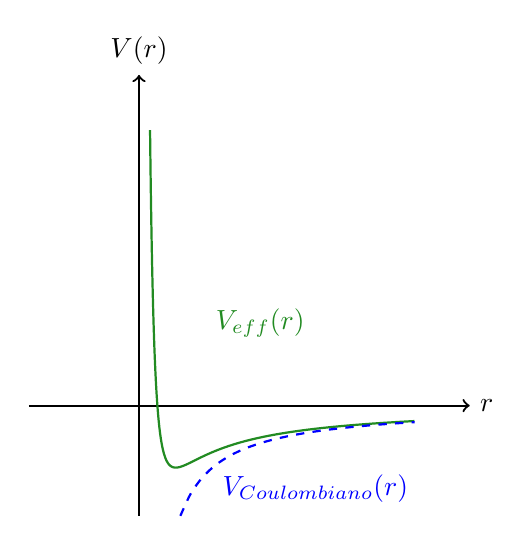
\begin{tikzpicture}[scale=0.7]

  	% Assi
 	 \draw[->, thick] (-2,0) -- (6,0) node[right] {$r$};
  	\draw[->, thick] (0,-2) -- (0,6) node[above] {$V(r)$};
	
	% Potenziale efficace: somma dei due 
  \draw[domain=0.2:5, smooth, thick, ForestGreen, samples = 500] plot (\x,{-1.5/(\x) + 0.5/(\x*\x)});

  	% Curva del potenziale coulombiano V(r) = -1/r
	\draw[domain=0.75:5, smooth, thick, dashed, blue] plot (\x,{-1.5/(\x)});
	
	% etichette
	% Etichetta della curva totale
 	\node[ForestGreen] at (2.2,1.5) {$V_{\text{eff}}(r)$};
	
	\node[blue] at (3.2,-1.5) {$V_{\text{Coulombiano}}(r)$};

	\end{tikzpicture}
	\end{center}
	%%%%%%%
	%%%%%%%
	
	\item Guardiamo ora le condizioni di accettabilità su $\chi$:
	
		Le soluzioni accettabili sono quelle che hanno norma convergente, ovvero:
	
	\begin{align*}
		\int_0^{\, +\infty} \dd r \, |\chi|^2 < \infty
	\end{align*}
	
		e ciò riporta tutto al problema di Schrodinger. Le soluzioni dell'equazione di Schrodinger devono essere infatti funzioni normalizzabili, quindi non tutte le soluzioni sono accettabili:
		
	\begin{align*}
		\int_{\mathbb{R}^3} \dd^3 x \, |\psi|^2 = \int_{S_2} \dd \Omega \int_0^{ \, + \infty} \dd r \, r^2 \psi^* \psi = \braket{Y} \int_0^{ \, + \infty} \dd r \, r^2 |R|^2 = |Y|^2 \int_0^{ \, + \infty} \dd r \, |\chi|^2 < \infty
	\end{align*}
	
		quindi per $ r \leq 0$ ho che vale $\chi\qty(r) = 0$. Ad ogni modo è comunque conveniente normalizzare $R$ e $Y$ separatamente:
		
	\begin{align*}
		\int_0^{ \, + \infty} |R|^2 \, r^2 \, \dd r = 1 \qquad ; \qquad \int_{0}^{2\pi} \int_0^{\pi} |Y|^2 \, \sin\theta \, \dd \theta \dd \phi = 1
	\end{align*}
	
\end{enumerate}

\subsection{Potenziale Coulombiano}

	Vediamo ora cosa accade per un \textit{potenziale Coulombiano.}
	\\
	\\
	Per $E \geq 0$ ho particelle libere, ovvero con uno spettro continuo. Per $E < 0$ ho particelle con stati legati, cioè con spettro discreto, quindi con stati normalizzabili. Mi concentro ora sugli spettri discreti negativi per il problema unidimensionale. Esiste quindi un unico stato con energia minima $\qty(l = 0)$ negativa, sotto al quale non vi sono soluzioni accettabili: è bene specificare che è necessario che tale minimo esista. Aumentando il valore di $l$, allora aumento anche l'energia $E$, poiché il potenziale efficace dipende dà $l$ stesso, quindi lo spettro unidimensionale è non degenere e la somma di tutti gli spettri da lo spettro del problema tridimensionale.
	\\
	\\
	In generale so che:
	
\begin{align*}
	\psi_{Elm}\qty(r, \theta, \phi) = R_{Elm}\qty(r) \, Y_{lm}\qty(\theta, \phi)
\end{align*}

	e che:
	
\begin{align*}	
	\chi_{El} \qty(r) = r \, R_{El}\qty(r)
\end{align*}

	perciò:
	
\begin{align*}
	\psi_{Elm} \qty(r, \theta, \phi) = \frac{\chi_{El}\qty(r)}{r} \, Y_{lm}\qty(\theta, \phi)
\end{align*}
	
	So che per $l$ fisso ho $2l + 1$ armoniche sferiche, pertanto per un valore fisso di energia $E$ ho:
	
\begin{itemize}
	\item $l = 0$
		
	\begin{align*}
		\psi_{E0m} = \psi_{E00} = \frac{\chi_{00}}{r} \, Y_{00} \, \, \Rightarrow \, \, \text{non ho degenerazione}
	\end{align*}

	\item $l = 1$
	
	\begin{align*}
		\psi_{E1m} = \qty{ \psi_{E1-1}, \psi_{E10}, \psi_{E11}} \, \, \Rightarrow \, \, \text{ho degenerazione $3$}
	\end{align*}
	
\end{itemize}

	La degenerazione non dipende quindi dalla parte radiale ma solo da quella angolare. Si osserva che:

\begin{align*}
	\qty[\hat{H}, \hat{L}_{\pm}] = 0 \quad ; \quad \qty[\hat{H}, \hat{L}_{3}] = 0 \quad ; \quad \qty[\hat{L}_{\pm}, \hat{L}_{3}] \neq 0 
\end{align*}

	il primo commutatore da un risultato molto importante: poiché $\hat{L}_{\pm}$ alza o abbassa il valore di $m$ poiché $\hat{L}_{\pm}$ commuta con $\hat{H}$, si ha che una variazione del valore di $m$ non influisce sul valore dell'energia: si parla di \textit{degenerazione essenziale.}
	\\
	\\
	Ci si aspetterebbe quindi che, per un livello che denoteremo $n$ di energia, ci siano $2l + 1$ stati degeneri (verificato prima): in realtà non è così in quanto sussiste un'ulteriore degenerazione tale per cui per ogni livello $n$, il valore di $l$ può variare da $0$ a $n - 1$. In questo caso si parla di \textit{degenerazione accidentale:} in generale, le degenerazioni accidentali non derivano dalla classe di problemi in generale, ma dalla particolare forma dell'Hamiltoniana presa in considerazione e, in particolare, dalla presenza del potenziale Coulombiano. Al livello $n$-esimo del potenziale coulombiano è associato un grado di degenerazione pari a:

\begin{align*}
	d\qty(n) = \sum_{ l = 0}^{n -1} \qty(2l  +1) = n^2
\end{align*}

	Vediamo ora cosa succede, per farci un'idea, per $l = 0$. In questo caso l'equazione di Schrodinger diventa, per il potenziale efficace Coulombiano:

\begin{nb}
\begin{align*}
	-\frac{\hbar^2}{2m} \, \chi_{n0}''\qty(r) - \frac{Z \, e^2}{4\pi \varepsilon_0 r} \, \chi_{n0}\qty(r) = E \, \chi_{n0}\qty(r)
\end{align*}
\end{nb}

	ovvero:
	
\begin{align*}
	- \chi_{n0}'' - \frac{2m \, Z \, e^2}{4\pi \, \varepsilon_0 \, r \hbar^2} \, \chi_{n0} = \frac{2mE}{\hbar^2} \, \chi_{n0}
\end{align*}

	Riscrivi adesso tutto in termini adimensionali, ossia $r = \rho a$, con $\rho$ quantità adimensionata e $a$ una lunghezza. In questo modo:
	
\begin{align*}
	\dv[2]{r} = \dv[2]{\qty(\rho a)} = \frac{1}{a^2} \, \dv[2]{\rho}
\end{align*}

	quindi derivando rispetto a $\rho$ e moltiplicando per $a^2$ si ha che:
	
\begin{align*}
	- \chi_{0}''\qty(\rho) - \frac{2m \, Z \, e^2}{4\pi \, \varepsilon_0 \hbar^2} \, \frac{a}{\rho} \, \chi_{0}\qty(\rho) = \frac{2ma^2}{\hbar^2} \, E \, \chi_{0}\qty(\rho)
\end{align*}

	dove il termine:
	
\begin{align*}
	\varepsilon \, \equiv \, \frac{2ma^2}{\hbar^2} \, E = \frac{E}{E_B} \, \, \Rightarrow \, \, E = \varepsilon \, E_B
\end{align*}

	è l'energia misurata rispetto all'energia di Bohr. Inoltre riconosco il raggio di Bohr al membro di sinistra e perciò:
	
\begin{align*}
	a_B = \frac{4\pi \, \hbar^2 \, \varepsilon_0}{me^2} \, \, \Rightarrow \,\, \frac{2mZ e^2}{4\pi \varepsilon_0 \hbar^2} \, \frac{a}{\rho} = \frac{2Z a}{a_{B \rho}}
\end{align*}

	da cui definisco:
	
\begin{align*}
	a \, \equiv \, \frac{a_B}{Z} = \frac{4 \pi \hbar^2 \, \varepsilon_0}{Z e^2 m} \, \, \Rightarrow \, \, \rho = \frac{Z r}{a_B}
\end{align*}

	che è proprio il raggio di Bohr per un \textbf{idrogeneide} $Z$.
	\\
	\\
	L'equazione si riduce quindi a:
	
\begin{align*}
	- \chi''\qty(\rho) - \frac{2}{\rho} \, \chi\qty(\rho) = \varepsilon \, \chi\qty(\rho)
\end{align*}
	
	la cui soluzione è del tipo:
	
\begin{align*}
	\chi\qty(\rho) = \rho \, e^{- c \rho}
\end{align*}

	che condizioni ho su $c$?
	\\
	\\
	Calcolando la derivata seconda della soluzione ed estraendo la derivata seconda dall'equazione per $\chi\qty(\rho)$, le metto a confronto ed ottengo:
	
\begin{align*}
	\rho c^2 - 2 c = \varepsilon \rho - 2
\end{align*}

	da cui, per confronto:

\begin{center}
\vspace{1em}
\begin{minipage}{0.25\textwidth}
\begin{empheq}[left = \empheqlbrace]{align*}
	& - \varepsilon = c^2 \\
	& -2c = -2 
\end{empheq}
\end{minipage}
\qquad $\Rightarrow$ \qquad
\begin{minipage}{0.25\textwidth}
\begin{empheq}[left = \empheqlbrace]{align*}
	& c = 1  \\
	& \varepsilon = -1
\end{empheq}
\end{minipage}
\vspace{1em}
\end{center}

	Poiché non ho nodi, per il teorema dei nodi, questo è lo stato di energia più bassa, quindi lo stato fondamentale sarà:
	
\begin{align*}
	\chi_{10}\qty(\rho) = \rho e^{ - \rho} = \frac{Z r}{a_B} \, e^{ \, - Zr/a_B}
\end{align*}

	e l'energia di questo stato è $E = - E_B = -13.6 \, \text{eV}$.
	\\
	\\
	Per il primo livello eccitato ($ n =2, l= 0$)?
	\\
	\\
	Ipotizzo una soluzione della forma:

\begin{align*}
	\chi\qty(\rho) = \qty(\rho + \alpha \rho^2) \, e^{ \, - c\rho}
\end{align*}

	per il primo livello eccitato. Calcolando le derivate analogamente a prima, andando a sostituire e verificando per confronto si ottiene:

\begin{center}
\vspace{1em}
\begin{minipage}{0.25\textwidth}
\begin{empheq}[left = \empheqlbrace]{align*}
	& - \varepsilon = c^2 \\
	& -2c = -2 
\end{empheq}
\end{minipage}
\qquad $\Rightarrow$ \qquad
\begin{minipage}{0.25\textwidth}

\begin{align*}
	\chi_{20} \qty(\rho) = \qty(\rho -\frac{1}{2} \, \rho^2) \, e^{ \, - 1/2 \, \rho}
\end{align*}

\end{minipage}
\vspace{1em}
\end{center}
	
	l'energia in questo caso è $E = - 1/4 \, E_B = - 3.4 \, \text{eV}$.

\section{L'Atomo di Idrogeno}

\begin{myapprf}
	\textbf{Che differenza c'è tra atomo di idrogeno ed atomo idrogeneide?}
	\\
	\\
	Sono diversi, infatti vale che:
	
\begin{itemize}
	\item \textit{Atomo di idrogeno:}
	
		Composto da:
		
	\begin{itemize}
		\item $1$ protone (nel nucleo),
			
		\item $1$ elettrone,
		
		\item è l’atomo più semplice dell’universo,
		
		\item simbolo: $\vb{H}$,
		
		\item descritto dalla meccanica quantistica con la ben nota soluzione dell’equazione di Schrödinger con potenziale coulombiano:
		\begin{align*}
			V\qty(r) = - \frac{e^2}{4\pi \varepsilon_0 r}
		\end{align*}

	\end{itemize}

	
	\item \textit{Atomo idrogeneide:}
	
		Composto da:
		
	\begin{itemize}
		\item Un solo elettrone, ma il nucleo può avere più protoni: $Z > 1$,
		\item Esempi:
		\begin{itemize}
			\item $\vb{He^+}$ (ione dell'elio con un elettrone $\to Z = 2$ ),
			\item $\vb{Li^{2+}}$ (ione del litio con un elettrone $\to Z = 3$).
		\end{itemize}

		\item In generale: sistemi a due corpi con:
		\begin{itemize}
			\item un elettrone, 
			\item un nucleo carico $+Z \, e$.
		\end{itemize}

	\end{itemize}
\end{itemize}

\end{myapprf}

	L'atomo di Idrogeno consiste di un protone pesante sostanzialmente fermo, di carica $e$, attorno al quale si trova un elettrone molto più leggero di carica $-e$. In questa approssimazione le due particelle interagiscono tramite un potenziale Coulombiano in cui poniamo $Z = 1$ ed indichiamo il raggio di Bohr senza pedice, ossia con $a$: trascuriamo quindi le correzioni relativistiche che comportano l'interazione "Spin - Orbita" (accoppiamento tra lo spin dell'elettrone ed il momento angolare orbitale del sistema) e "Spin - Spin" (accoppiamento tra gli spin di elettrone e protone), pertanto avremo un'Hamiltoniana indipendente dallo spin. Se indichiamo una base dell'insieme completo di osservabili $\qty{\hat{H}, \hat{L}^2, \hat{L}_3}$ con $\ket{n \, l \, m}$ che ricordiamo essere tali che:
	
\begin{empheq}[left = \empheqlbrace]{align*}
	& n = 1, 2, 3, \ldots \\
	& l = 0, \ldots, n -1 \\
	& m = -l, -l +1, \ldots, l- 1, l
\end{empheq}

	allora l'equazione di Schrodinger la scriviamo come:
	
\begin{align*}
	\hat{H} \psi_{nlm} \qty(r, \theta, \phi) = E_n \psi_{nlm}\qty(r, \theta, \phi)
\end{align*}

	la cui soluzione più generale è come sappiamo:
	
\begin{align*}
	\psi_{nlm}\qty(r, \theta, \phi) = R_{nl}\qty(r) \, Y_{l}^m\qty(\theta, \phi)
\end{align*}

\begin{myapprf}
	Ricordiamo che $R$ è la parte radiale, $Y$ la parte angolare, in particolare:
	
\begin{itemize}
	\item $R_{nl}\qty(r)$: funzione radiale, contiene l'informazione su come varia la probabilità dell’elettrone con la distanza dal nucleo.
	
	\item $Y_{l}^m\qty(\theta, \phi)$:  armoniche sferiche, contengono la dipendenza angolare.
\end{itemize}

\end{myapprf}

	Poiché il caso dell'atomo di idrogeno è il caso più semplice in assoluto di idrogeneide, tutti i discorsi fatti nella sezione precedente sono ancora validi. In particolare, la quantizzazione delle energie dell'atomo idrogeneide è data dalla seguente formula:
	
\begin{mydef}
	Definiamo la \textbf{formula di Bohr estesa}:

\begin{align*}
	E_n = - \qty[\, \frac{m}{2\hbar^2} \, \qty(\frac{Z \, e^2}{4\pi\varepsilon_0})^2   \,] \, \frac{1}{n^2} = \frac{E_1}{n^2} \, Z^2 = - \frac{13.6 \, \text{eV}}{n^2} \, Z^2
\end{align*}

	che per $Z = 1$ da l'energie dell'atomo di Idrogeno.

\end{mydef}

	È immediato verificare che i valori di energia trovati prima nell'esempio di $l = 0$, tramite $E = \varepsilon E_B$, sono corretti. Si ha quindi che l'\textbf{energia di legame} dell'Idrogeno (la quantità di energia necessaria da fornire all'elettrone nello stato fondamentale in modo da ionizzare l'atomo) è $13.6 \, \, \text{eV}$.
	\\
	\\
	Proviamo a trovare la funzione d'onda relativa allo stato fondamentale dell'atomo di Idrogeno. Per separazione delle variabili abbiamo visto che:
	
\begin{align*}
	\psi_{100} \qty(r, \theta, \phi) = R_{10}\qty(r) \, Y_0^0\qty(\theta, \phi)
\end{align*}

	e dall'equazione per $\chi_{10}\qty(r)$ si ha che:
	
\begin{align*}
	R_{10}\qty(r) = \frac{c_0}{a} \, e^{\, -r/a}
\end{align*}

	dove $c_0$ indica il fattore di normalizzazione. Tocca ora normalizzare la parte radiale, quindi:
	
\begin{align*}
	\int_0^{\, +\infty} |R_{10}|^2 \, r^2 \, \dd r = \frac{|c_0|^2}{a^2}\int_0^{\, +\infty} e^{\, -2r/a} \, r^2 \, \dd r = |c_0|^2 \, \frac{a}{4} = 1 \, \, \Rightarrow \, \, c_0 = \frac{2}{\sqrt{a}}
\end{align*}

	Dall'equazione per le armoniche sferiche troviamo invece che: $Y_0^0 = 1/\sqrt{4\pi}$, pertanto:
	
\begin{align*}
	\psi_{100}\qty(r, \theta, \phi) = \frac{1}{\sqrt{\pi a^3}} \, e^{\, -r/a}
\end{align*}

	Se passo al livello successivo, $n = 2$, l'energia è:
	
\begin{align*}
	E_2 = - \frac{13.6 \,\, \text{eV}}{4} = - 3.4 \, \, \text{eV}
\end{align*}

	questa è l'energia del primo stato eccitato, o meglio dei primi stati eccitati, dal momento che per $n = 2$ possiamo avere $ l=0$ (in cui $m = 0$) e $l=1$(in cui $m=-1, 0, +1$): si hanno quindi $4$ stati che condividono la stessa energia. Per un valore qualsiasi di $n$ abbiamo che $l$ va da $0$ a $n-1$ e per ogni valore di $l$ si hanno $2l + 1$ possibili valori di $m$, perciò come già detto in precedenza, la degenerazione del livello energetico $E_n$ è:
	
\begin{align*}
	d\qty(n) = \sum_{l = 0}^{n-1} \qty(2l + 1) = 2 \, \sum_{l = 0}^{n-1} l +  \sum_{l = 0}^{n-1} 1 = 2 \, \frac{1}{2} \, \qty(n -1) \, \qty(n -1 + 1) + n = n^2
\end{align*}
	
	In generale si potrebbe ricavare qualsiasi funzione d'onda dell'Idrogeno col metodo per gli idrogeneidi e successiva normalizzazione, ma diventerebbe estremamente lungo e complicato. Senza darne una dimostrazione si da la seguente definizione:
	
\begin{mydef}
	
	Si ha che le \textcolor{red}{\textbf{funzioni d'onda spaziali normalizzate dell'Idrogeno}} in questa approssimazione sono date da:

\begin{align*}	
		\textcolor{red}{\psi_{nlm}\qty(r, \theta, \phi)} = \sqrt{   \qty( \frac{2}{na} )^3 \, \frac{\qty(n - l - 1)!}{ 2n \, \qty[\qty(n+l)!]^3}   } \, e^{ \, - r/\qty(na)} \, \qty(\frac{2r}{na})^l \, \qty[ L_{n-l-1}^{2l+1} \, \qty(\frac{2r}{na} ) ] \, Y_l^m \qty(\theta, \phi)
\end{align*}

	dove la funzione $L^p_{q-p}\qty(x)$ è un \textcolor{blue}{\textbf{polinomio di Laguerre associato}}, definito come:
	
\begin{align*}
	\textcolor{blue}{L_{q-p}^p \qty(x) }= \qty(-1)^p \, \qty(\dv{x})^q \, L_q\qty(x)
\end{align*}
	
	in cui il \textcolor{cyan}{\textbf{$q$-esimo polinomio di Laguerre}} è:

\begin{align*}
	\textcolor{cyan}{  L_q\qty(x)  } = e^x \, \qty(\dv{x})^q \, \qty(e^{\, -x} \, e^{q})
\end{align*}

\end{mydef}

	Inoltre vale che le funzioni d'onda sono mutuamente ortogonali, ovvero:
	
\begin{align*}
	\int \psi_{nlm}^* \, \psi_{n' l' m'} \, r^2 \sin\theta \, \dd r \dd \theta \dd \phi = \delta_{nn'} \, \delta_{ll'} \, \delta_{mm'}
\end{align*}

	cioè segue dall'ortogonalità delle armoniche sferiche e dal fatto che (per $n \neq n'$) esse sono autofunzioni di $\hat{H}$ on autovalori distinti. Per dare un'idea circa il comportamento della funzione d'onda, si mostra un grafico delle prime funzioni radiali $R_{nl}$:

\begin{figure}[H]
  	\centering
	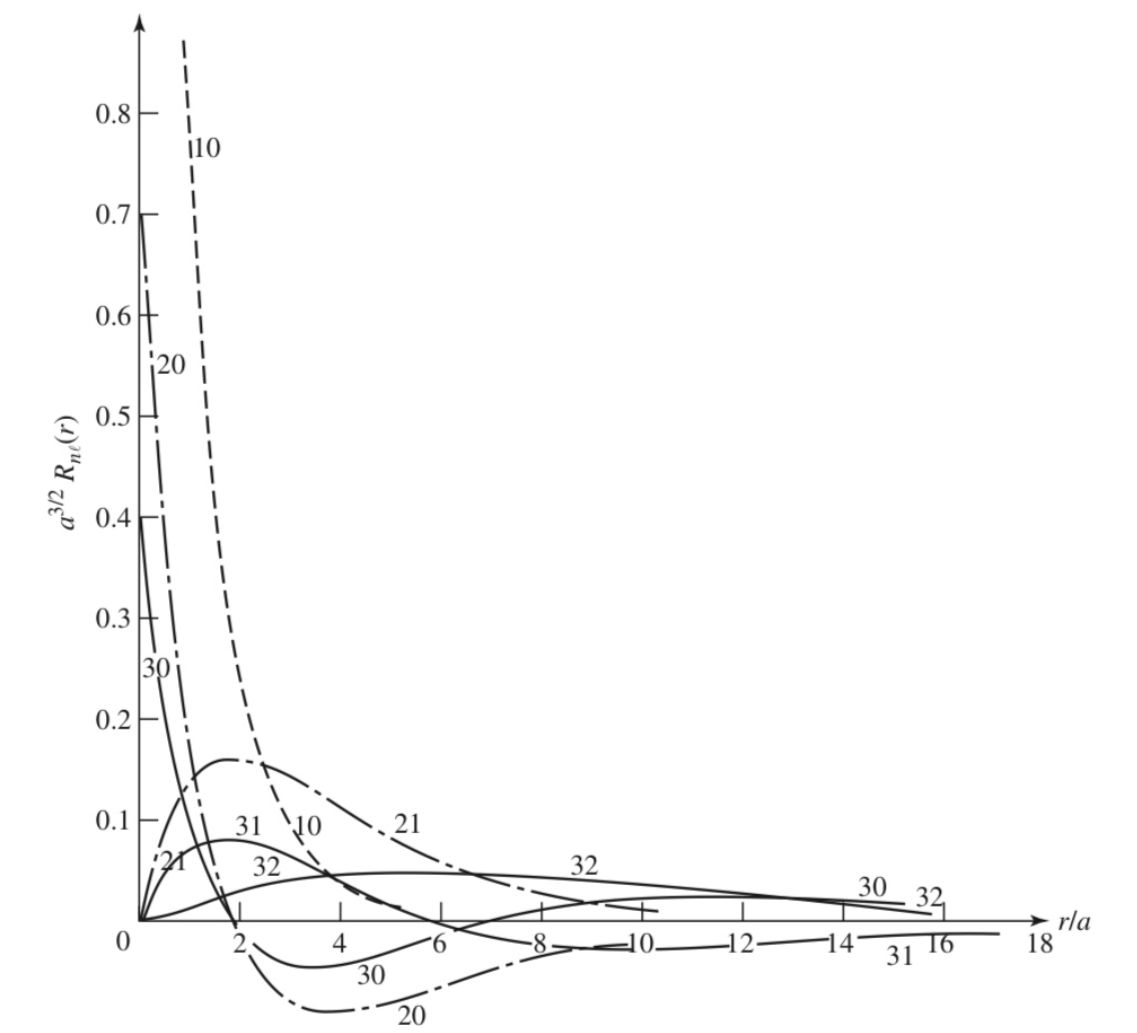
\includegraphics[width = 0.7 \textwidth]{chapter5/section3/imm/imm1.jpg}
\end{figure}

	Un modo invece di visualizzare l'intera funzione d'onda consiste nelle \textit{nubi di densità} in cui la luminosità della nube è proporzionale a $|\psi|^2$:

\begin{figure}[H]
  	\centering
	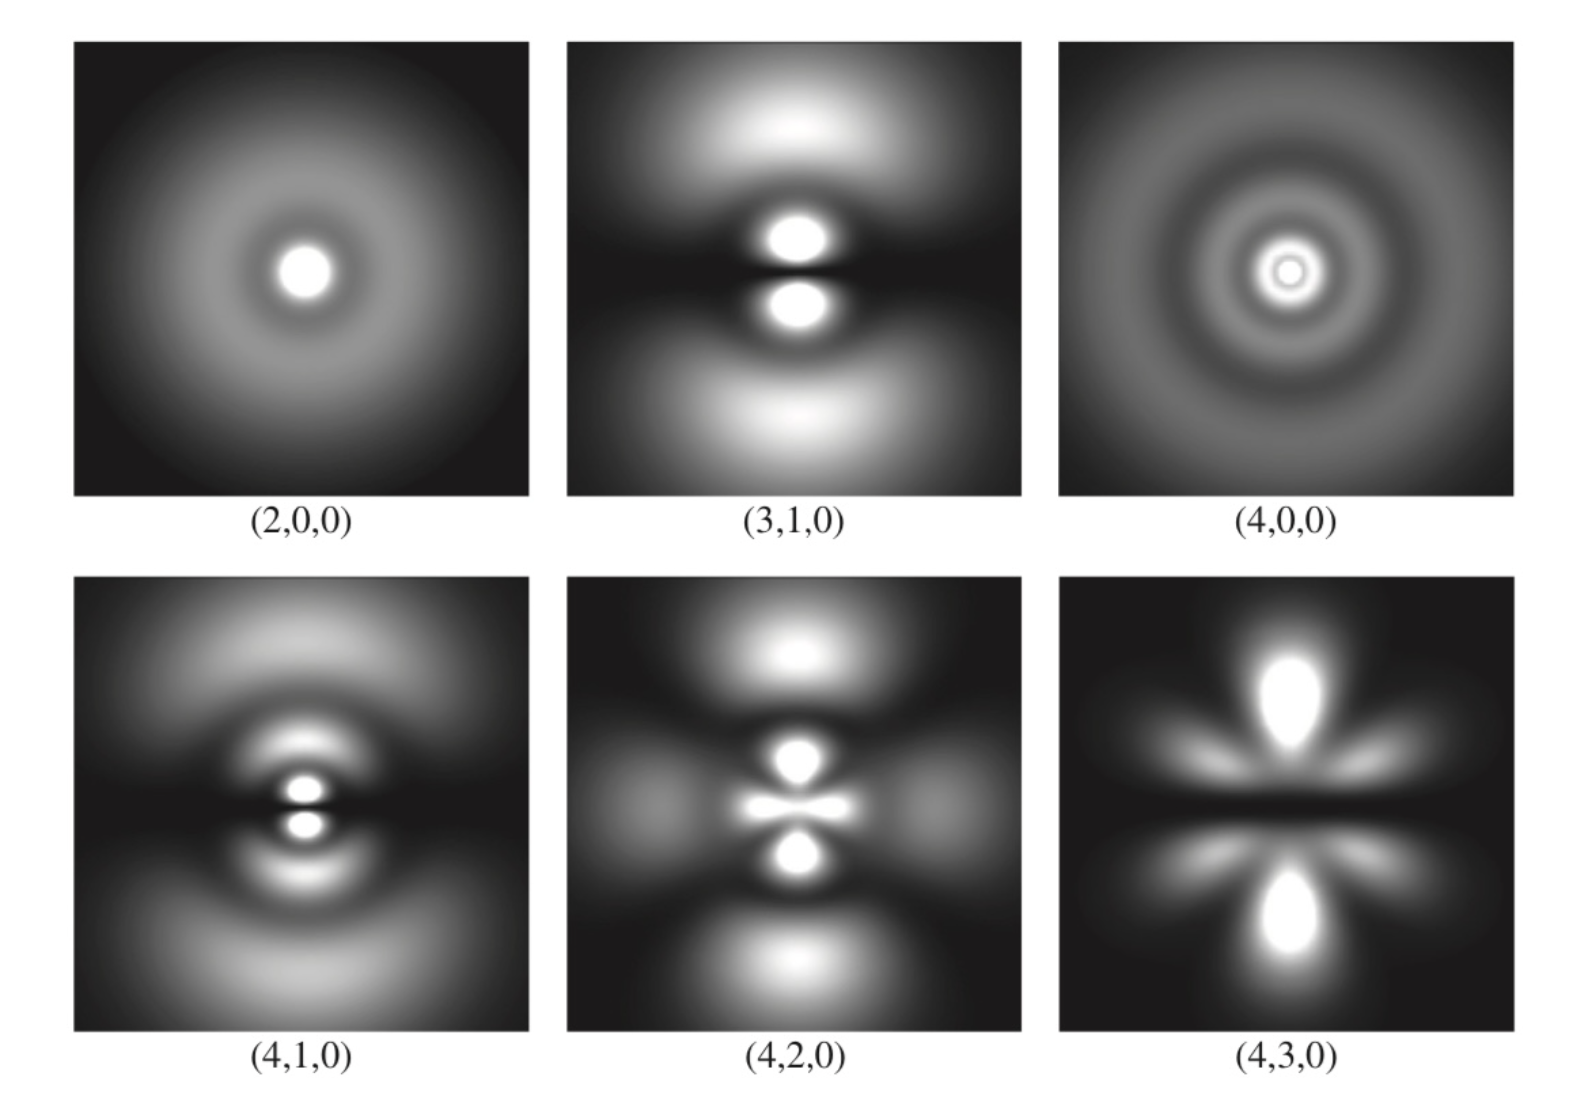
\includegraphics[width = 0.75 \textwidth]{chapter5/section3/imm/imm2.jpg}
\end{figure}

	mentre un modo alternativo più quantitativo ma più difficile da visualizzare, consiste nelle \textit{superfici con densità di probabilità costante}, ovvero:
	
\begin{figure}[H]
  	\centering
	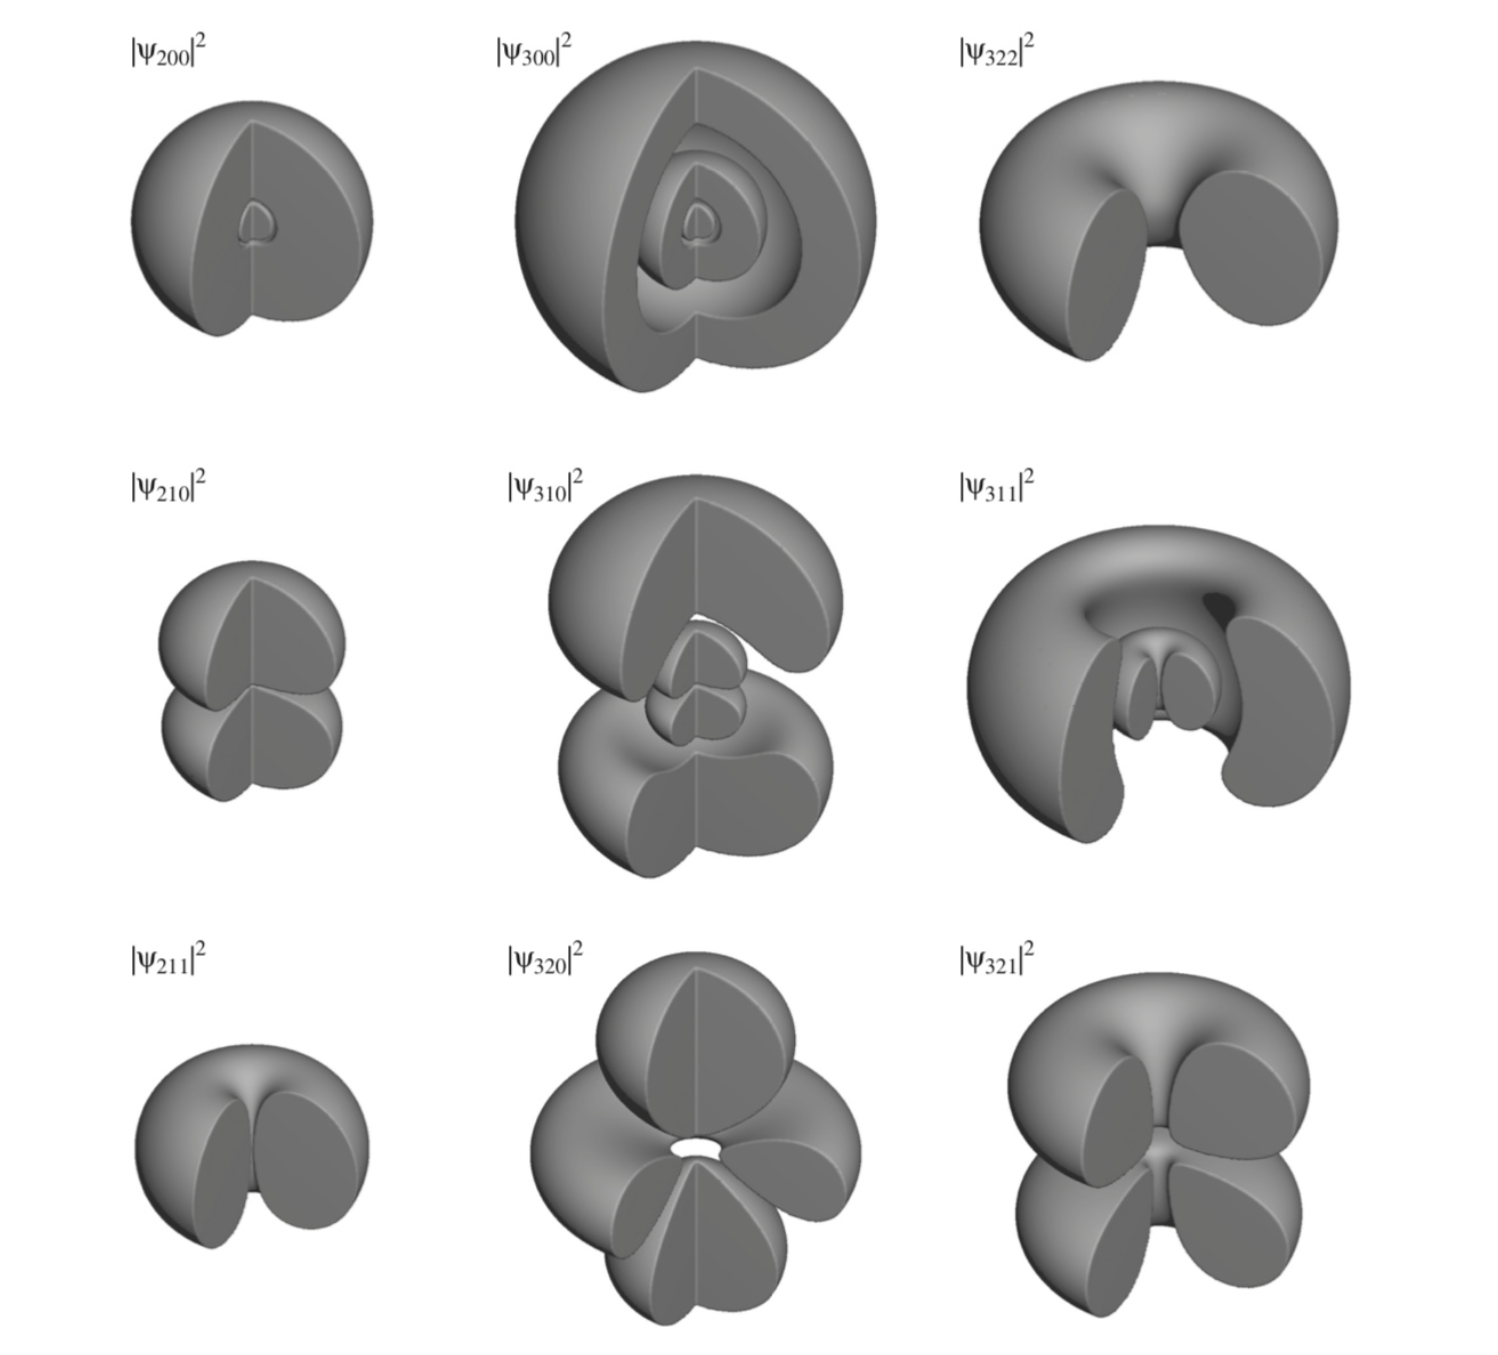
\includegraphics[width = 0.86 \textwidth]{chapter5/section3/imm/imm3.jpg}
\end{figure}

	Per concludere il discorso sull'atomo di Idrogeno facciamo un'ultima considerazione: come teniamo conto del fatto che l'elettrone ha uno spin?
	\\
	\\
	Se l'Hamiltoniana non dipende esplicitamente dallo spin allora una generica funzione d'onda, nella base degli autostati:
	
\begin{align*}
	\ket{n \, l \, m \, \sigma}
\end{align*}

	con $\sigma$ che indica la proiezione dello spin sull'asse $z$, sarà espressa come il prodotto tra la funzione d'onda orbitale $\psi_{nlm}$ ed una combinazione lineare dei vettori della base dello spin $1/2$, $\qty{\ket{+} \, \ket{-}}$, ossia:
	
\begin{align*}
	\Psi_{nlm}\qty(r, \theta, \phi, \sigma) = \alpha \, \psi_{nlm} \qty(r, \theta, \phi) \ket{+} + \beta \, \psi_{nlm}\qty(r, \theta, \phi) \ket{-}
\end{align*}

	scritta anche come:
	
\begin{align*}
	\Psi_{nlm} \qty(r, \theta, \phi, \sigma) = \mqty( \alpha \, \psi_{nlm} \qty(r, \theta, \phi, +) \\  \beta \, \psi_{nlm} \qty(r, \theta, \phi, -) )
\end{align*}

	pertanto ogni stato dell'atomo di Idrogeno ha una degenerazione pari a $2n^2$: per ogni $n, l, m$ fissati ho una degenerazione spaziale $n^2$, a cui però va aggiunta la degenerazione di spin che è $2$, che deriva dalla possibilità di avere spin up oppure spin down. In modo del tutto simile, se considerassimo anche la presenza dello spin protonico, avremmo un ulteriore fattore $2$ di degenerazione di spin, portando la degenerazione complessiva ad essere $4n^2$.






